%File: anonymous-submission-latex-2024.tex
\documentclass[letterpaper]{article} % DO NOT CHANGE THIS
\usepackage[submission]{aaai24}  % DO NOT CHANGE THIS
\usepackage{times}  % DO NOT CHANGE THIS
\usepackage{helvet}  % DO NOT CHANGE THIS
\usepackage{courier}  % DO NOT CHANGE THIS
\usepackage[hyphens]{url}  % DO NOT CHANGE THIS
\usepackage{graphicx} % DO NOT CHANGE THIS
\urlstyle{rm} % DO NOT CHANGE THIS
\def\UrlFont{\rm}  % DO NOT CHANGE THIS
\usepackage{natbib}  % DO NOT CHANGE THIS AND DO NOT ADD ANY OPTIONS TO IT
\usepackage{caption} % DO NOT CHANGE THIS AND DO NOT ADD ANY OPTIONS TO IT
\frenchspacing  % DO NOT CHANGE THIS
\setlength{\pdfpagewidth}{8.5in} % DO NOT CHANGE THIS
\setlength{\pdfpageheight}{11in} % DO NOT CHANGE THIS
%
% These are recommended to typeset algorithms but not required. See the subsubsection on algorithms. Remove them if you don't have algorithms in your paper.
\usepackage{algorithm}
\usepackage{algorithmic}

%
% These are are recommended to typeset listings but not required. See the subsubsection on listing. Remove this block if you don't have listings in your paper.
\usepackage{newfloat}
\usepackage{listings}
\DeclareCaptionStyle{ruled}{labelfont=normalfont,labelsep=colon,strut=off} % DO NOT CHANGE THIS
\lstset{%
	basicstyle={\footnotesize\ttfamily},% footnotesize acceptable for monospace
	numbers=left,numberstyle=\footnotesize,xleftmargin=2em,% show line numbers, remove this entire line if you don't want the numbers.
	aboveskip=0pt,belowskip=0pt,%
	showstringspaces=false,tabsize=2,breaklines=true}
\floatstyle{ruled}
\newfloat{listing}{tb}{lst}{}
\floatname{listing}{Listing}
%
% Keep the \pdfinfo as shown here. There's no need
% for you to add the /Title and /Author tags.




\usepackage{booktabs}
\usepackage{multirow}
\usepackage{xspace}
% \usepackage{hyperref}
\usepackage{xcolor}
\newcommand{\tuple}[1]{\ensuremath{\langle #1\rangle}}
% \newcommand{\Omri}[1]{\textcolor{orange}{\textsc{Omri}: #1}}
% \newcommand{\Carmel}[1]{\textcolor{red}{\textsc{Carmel}: #1}}
% \newcommand{\Roni}[1]{\textcolor{green}{\textsc{Roni}: #1}}
\newcommand{\Omri}[1]{}
\newcommand{\Carmel}[1]{}
\newcommand{\Roni}[1]{}
\newcommand{\shortcite}[1]{\cite{#1}}
\newcommand{\gtv}[1]{\ensuremath{\textit{G2V}}\xspace}
\newcommand{\fgtv}[1]{\ensuremath{\textit{FG2V}}\xspace}
\newcommand{\kaduri}[1]{\ensuremath{\textit{KBS}}\xspace}
\newcommand{\mapfgas}[1]{\ensuremath{\textit{MAG}}\xspace}
\newtheorem{example}{Example}










\usepackage{colortbl}
\definecolor{Gray}{gray}{0.9}





% DISALLOWED PACKAGES
% \usepackage{authblk} -- This package is specifically forbidden
% \usepackage{balance} -- This package is specifically forbidden
% \usepackage{color (if used in text)
% \usepackage{CJK} -- This package is specifically forbidden
% \usepackage{float} -- This package is specifically forbidden
% \usepackage{flushend} -- This package is specifically forbidden
% \usepackage{fontenc} -- This package is specifically forbidden
% \usepackage{fullpage} -- This package is specifically forbidden
% \usepackage{geometry} -- This package is specifically forbidden
% \usepackage{grffile} -- This package is specifically forbidden
% \usepackage{hyperref} -- This package is specifically forbidden
% \usepackage{navigator} -- This package is specifically forbidden
% (or any other package that embeds links such as navigator or hyperref)
% \indentfirst} -- This package is specifically forbidden
% \layout} -- This package is specifically forbidden
% \multicol} -- This package is specifically forbidden
% \nameref} -- This package is specifically forbidden
% \usepackage{savetrees} -- This package is specifically forbidden
% \usepackage{setspace} -- This package is specifically forbidden
% \usepackage{stfloats} -- This package is specifically forbidden
% \usepackage{tabu} -- This package is specifically forbidden
% \usepackage{titlesec} -- This package is specifically forbidden
% \usepackage{tocbibind} -- This package is specifically forbidden
% \usepackage{ulem} -- This package is specifically forbidden
% \usepackage{wrapfig} -- This package is specifically forbidden
% DISALLOWED COMMANDS
% \nocopyright -- Your paper will not be published if you use this command
% \addtolength -- This command may not be used
% \balance -- This command may not be used
% \baselinestretch -- Your paper will not be published if you use this command
% \clearpage -- No page breaks of any kind may be used for the final version of your paper
% \columnsep -- This command may not be used
% \newpage -- No page breaks of any kind may be used for the final version of your paper
% \pagebreak -- No page breaks of any kind may be used for the final version of your paperr
% \pagestyle -- This command may not be used
% \tiny -- This is not an acceptable font size.
% \vspace{- -- No negative value may be used in proximity of a caption, figure, table, section, subsection, subsubsection, or reference
% \vskip{- -- No negative value may be used to alter spacing above or below a caption, figure, table, section, subsection, subsubsection, or reference

\setcounter{secnumdepth}{0} %May be changed to 1 or 2 if section numbers are desired.

% The file aaai24.sty is the style file for AAAI Press
% proceedings, working notes, and technical reports.
%

% Title

% Your title must be in mixed case, not sentence case.
% That means all verbs (including short verbs like be, is, using,and go),
% nouns, adverbs, adjectives should be capitalized, including both words in hyphenated terms, while
% articles, conjunctions, and prepositions are lower case unless they
% directly follow a colon or long dash
\title{Algorithm Selection for Optimal Multi-Agent Path Finding via Graph Embedding}
\author{
    %Authors
    % All authors must be in the same font size and format.
    Written by AAAI Press Staff\textsuperscript{\rm 1}\thanks{With help from the AAAI Publications Committee.}\\
    AAAI Style Contributions by Pater Patel Schneider,
    Sunil Issar,\\
    J. Scott Penberthy,
    George Ferguson,
    Hans Guesgen,
    Francisco Cruz\equalcontrib,
    Marc Pujol-Gonzalez\equalcontrib
}
\affiliations{
    %Afiliations
    \textsuperscript{\rm 1}Association for the Advancement of Artificial Intelligence\\
    % If you have multiple authors and multiple affiliations
    % use superscripts in text and roman font to identify them.
    % For example,

    % Sunil Issar\textsuperscript{\rm 2},
    % J. Scott Penberthy\textsuperscript{\rm 3},
    % George Ferguson\textsuperscript{\rm 4},
    % Hans Guesgen\textsuperscript{\rm 5}
    % Note that the comma should be placed after the superscript

    1900 Embarcadero Road, Suite 101\\
    Palo Alto, California 94303-3310 USA\\
    % email address must be in roman text type, not monospace or sans serif
    proceedings-questions@aaai.org
%
% See more examples next
}

%Example, Single Author, ->> remove \iffalse,\fi and place them surrounding AAAI title to use it
\iffalse
\title{My Publication Title --- Single Author}
\author {
    Author Name
}
\affiliations{
    Affiliation\\
    Affiliation Line 2\\
    name@example.com
}
\fi

\iffalse
%Example, Multiple Authors, ->> remove \iffalse,\fi and place them surrounding AAAI title to use it
\title{My Publication Title --- Multiple Authors}
\author {
    % Authors
    First Author Name\textsuperscript{\rm 1},
    Second Author Name\textsuperscript{\rm 2},
    Third Author Name\textsuperscript{\rm 1}
}
\affiliations {
    % Affiliations
    \textsuperscript{\rm 1}Affiliation 1\\
    \textsuperscript{\rm 2}Affiliation 2\\
    firstAuthor@affiliation1.com, secondAuthor@affilation2.com, thirdAuthor@affiliation1.com
}
\fi


% REMOVE THIS: bibentry
% This is only needed to show inline citations in the guidelines document. You should not need it and can safely delete it.
\usepackage{bibentry}
% END REMOVE bibentry

\begin{document}

\maketitle

\begin{abstract}
Multi-agent path finding (MAPF) is the problem of finding paths for multiple agents such that they do not collide.
Finding optimal solutions to MAPF is NP-Hard, yet modern optimal solvers can scale to hundreds of agents and even thousands in some cases.
Different solvers employ different approaches, and there is no single state-of-the-art approach for all problems.
Furthermore, there are no clear, provable, guidelines for choosing when each optimal MAPF solver to use.
Prior work employed Algorithm Selection (AS) techniques to learn such guidelines from past data.
A major challenge when employing AS for choosing an optimal MAPF algorithm is how to encode the given MAPF problem.
Prior work either used hand-crafted features, graph embedding of the shortest paths, or an image representation of the problem. Each encoding is lossy, in the sense that it does not capture some aspect of the MAPF problem.
We propose a graph encoding of the MAPF problem and show how it can be used on-the-fly with a modern graph embedding algorithm called FEATHER.
We also show how this encoding can be effectively joined with existing encodings, resulting in a novel AS method we call MAPF Algorithm selection via Graph embedding (\mapfgas\ ). An extensive experimental evaluation of \mapfgas\ on several MAPF algorithm selection tasks reveals that it outperforms existing methods significantly.
\end{abstract}

\section{Introduction}
\label{scn:Intro}
%TO FIX (copied from KAduri Experimental Evaluation)

Multi-Agent Path Finding (MAPF) is the problem of finding paths for a group of agents, moving each agent from its initial location to a designated target location.
The main constraint in MAPF is that the agents must not collide.
% Applications
MAPF has received significant interest recently in the scientific community and in industry, as it has applications in robotics~\cite{veloso2015cobots} and automated warehouses~\cite{wurman2008coordinating}.
Finding an optimal solution to MAPF with respect to various optimization criteria, is known to be NP Hard~\cite{anOptimization2010surynek,structure2013yu}.
Nevertheless, a range of practical algorithms that guarantee optimality exists~\cite{kornhauser1984pebble,surynek2009novel}.
It has been shown that these algorithms are able to find optimal solutions to MAPF problems with more than 100 agents with less than one minute of runtime~\cite{li2021pairwise}.

% Different approaches work in different places
Different optimal MAPF algorithms employ different problem-solving techniques. For example, EPEA*~\cite{goldenberg2014enhanced} employs a heuristic search technique, BCP~\cite{lam2022branch} uses optimization techniques, and SAT-MDD~\cite{surynek2016efficient} compiles MAPF to Boolean Satisfiability.
% Appropriately choosing the right MAPF solver can allow finding provably optimal solutions to MAPF problems with more than 100 agents with less than one minute of runtime~\cite{li2021pairwise}.
Correspondingly, different solvers work best for different MAPF instances, and no algorithm has emerged to dominate all others.
The variance in performance can be great, where some algorithms perform poorly on some instances but significantly outperform all others on other instances.
On a recently performed extensive comparison of 5 optimal MAPF algorithms~\cite{kaduri2021experimental}, it was shown that even the least effective algorithm had some grids in which it was able to solve instances with 4 times more agents than all other evaluated algorithms. % SAT-MDD
Thus, developing methods for selecting the best optimal MAPF search algorithm for a given instance is a worthwhile endeavor. % UP to here edits


% the algorithm performing
% Kaduri et al.~\shortcite{kaduri2021experimental}
% performed an extensive comparison of 5 optimal MAPF algorithms
% showed that the SAT-MDD algorithm is the fastest
% is the fastest showed that SAT-MDD solves on some grids 4 times mor the performance of


The problem of determining which algorithm from a given set of algorithms is expected to perform best on a given problem instance is known as the
Algorithm Selection (AS) problem~\cite{rice1976algorithm,kerschke2019automated}.\footnote{Technically, this problem is called the \emph{per-instance AS} problem.}
Several recent works have developed AS techniques for optimal MAPF~\cite{kaduri2020algorithm,ren2021mapfast,alkazzi2022mapfaster}.
They used supervised learning to
train a classifier that chooses the best optimal MAPF algorithm for a given MAPF instance, from a portfolio of optimal MAPF algorithms that include EPEA*~\cite{goldenberg2014enhanced}, ICTS~\cite{sharon2013increasing}, SAT-MDD~\cite{surynek2016efficient}, CBSH~\cite{felner2018adding}, and Lazy CBS~\cite{gange2019lazy}.
%\Carmel{algorithms portfolio is missing in paper?} \Roni{Not sure what you mean. I just added above also the reference for MAPFAST if that's what you were saying} \Carmel{I meant introduce the solvers in our dataset} RONI: DONE
% While they achieved remarkable results, their algorithm portfolio only included search-based MAPF algorithm. Specifically, they did not consider using MDD-SAT or Lazy CBS. \Roni{MAPFASTER also included SAT and BCP (but not Lazy CBS as far as I can tell}
A key challenge faced by all prior work on AS for optimal MAPF is how to encode a given MAPF instance, as an input to the supervised learner. Prior works proposed hand-crafted MAPF-related features, casting the MAPF instance as an image~\cite{alkazzi2022mapfaster}, and graph embedding of a subgraph containing the shortest paths from start to target. Neither of these encodings completely captures the encoded MAPF instance.



To this end, we propose several contributions.
The first contribution is a different encoding of the MAPF instance called \fgtv\ , that fully utilizes the power of graph embedding algorithms by encoding the entire graph, augmented with artificial edges marking the start and target vertices of every agent.
This embedding is done using FEATHER~\cite{rozemberczki2020characteristic}, a modern graph embedding algorithm. %\Roni{Maybe there is something interesting about how we trained it in our context}
The resulting embedding yields superior results in most cases, but not always.
The second contribution is a simple method for integrating multiple encodings, which enables a more comprehensive encoding of the problem. This method can be used with different embeddings in a seamless manner. The resulting AS method is called \mapfgas\ .
Our third contribution is a comprehensive evaluation of \mapfgas\ on a standard benchmark over three different AS tasks, which differ in how similar are the train and test instances. Our results show that \mapfgas\ is superior to baseline methods, demonstrating the first practical AS method for MAPF that utilizes graph embeddings. All our code and datasets will be made publicly available to the community.

% We compared experimentally the different AS algorithms on a standard optimal MAPF dataset. Our results show that ....
% \Roni{detail our results}

%FROM MAPFASTER: The proposed portfolio contains Search-Based algorithms: CBS [25], CBSH [27], an Optimization-Based algorithm: BCP [28], and a Satisfiability-Based algorithm: SAT [29]

% Recently, a benchmark of MAPF problems in grid environments
% have been proposed (Stern et al. 2019), which includes a diverse set of XX grids. another more recent benchmark proposed (by Jingyao Ren) which includes a diverse set of XX grids from defrent grid types



\section{Background}
\label{scn:Background}


For completeness, we provide here a brief background on MAPF, AS for MAPF, and graph embedding.

\subsection{MAPF}
A MAPF problem instance is defined by a tuple $\tuple{k,G,s,t}$
where
$k$ is the number of agents,
$G = (V;E)$ is an undirected graph,
$s: [1\ldots, k]\rightarrow V$ maps an agent to its source vertex,
and $t: [1,\ldots, k]\rightarrow V$ maps an agent to its target vertex.
Initially, each agent is in its source vertex.
In every time step, each agent either waits
in its current vertex or moves to one of the vertices adjacent to it.
A single-agent plan for agent $i$ is a sequence of move/wait actions that moves $i$ from $s(i)$ to $t(i)$.
A solution to a MAPF instance is a set of single-agent plans, one for each agent, such that the agents do not collide with each other.
In the classical MAPF problem, the cost of a solution is either the sum of actions in all single-agent plans
or the number of actions in the longest single-agent plan. The former cost function is known as sum-of-costs (SOC) and the latter is known as makespan.
We measured solution cost in terms of SOC in our experiments, but most of our contributions are agnostic to the chosen cost function.
MAPF extensions that consider non-unit action costs, large agents, and continuous time have been explored~\cite{atzmon2020generalizing,andreychuk2022multi,li2019multi}. In this work, we focus on classical MAPF.


Optimal classical MAPF algorithms are classical MAPF algorithms that are guaranteed to return optimal solutions according to a predefined solution cost function.
Different optimal algorithms have been proposed for solving classical MAPF problems.
Prime examples are EPEA*~\cite{goldenberg2014enhanced}, SAT-MDD~\cite{anOptimization2010surynek}, CBS~\cite{sharon2015conflict,felner2018adding} and its many extensions, BCP~\cite{lam2022branch}, Lazy CBS~\cite{gange2019lazy}, and ICTS~\cite{sharon2013increasing}. These algorithms apply a range of techniques: some use heuristic search on dedicated state spaces, other compile the problem to Boolean Satisfiability (SAT) and call an off-the-shelf SAT solver, while others borrow ideas from constraint programming.
No algorithm fully dominates the other, and different  problems are solved best with different algorithms. This raised the need for an automated way to select which optimal MAPF solver to use for a given problem.




\subsection{AS for MAPF}



Previously proposed AS methods for MAPF followed a standard supervised learning paradigm,
and differ mainly in the type of features they extract.
Sigurdson et al.~\cite{sigurdson2019automatic} and Ren et al.~\cite{ren2021mapfast} mapped a given MAPF problem to an image and extracted image-based features with a Convolutional Neural Networks (CNN).
Kaduri, Boyarski, and Stern~\cite{kaduri2020algorithm} proposed a set of hand-crafted, MAPF-specific features, such as the number of agents divided
by the number of unblocked cells in the grid.
We refer to these features as the \kaduri\ features.
Ren et al. also explored the potential of using features that are based on mapping the given MAPF problem to a graph and using a \emph{graph embedding} method.
While their exploration showed that graph embedding can provide useful features for MAPF AS, they do not provide a practical method to use it. In fact, they consider their method to be ``not a deployable algorithm selector in any reasonable sense''~\cite{ren2021mapfast}, since it could not be used on any MAPF problem not observed during training.
We overcome this limitation in our work.
 \Carmel{this sentence is very misleading, for example Kaduri method can be deployed it can be used on problems/maps that are not part of train}\Roni{But this sentence is about the G2V method. They wrote it themselves (it's a quote). I rephrased a bit after your comment to make it clearer. Let me know if you're happy or not with it.}
%\Roni{Maybe even pull this to the intro. Let me think about it}


%Therefore, it is not a deployable algorithm selector in any reasonable sense.


Kaduri et al.~\cite{kaduri2021experimental} distinguished between three types of AS problems for MAPF:
(1) in-grid AS, (2) in-grid-type, and (3) between-grid-type.
In-grid AS means the train and test problems are all from the same underlying graph.
In-grid-type means the train and test problems are on different grids, but their grids have similar topologies.
\Carmel{more accurate - In-grid-type means the train and test problems are from the same grid types but totally different maps}
\Roni{I rephrased}
Between-grid-type means that graphs in the train and test problems are completely different, e.g., training on maze-like graphs and testing on graphs that represent road map in a city. Most prior work has focused on the in-grid AS problem, which is, of course, significantly easier.


% Therefore, it is not a deployable algorithm
% selector in any reasonable sense

% While their results were encouraging, they could not apply  to extract a vector representation of. We describe th


% extracting
% specifically designed for MAPF, and demonstrated their use in an AS method for optimal MAPF.

% to select suboptimal MAPF algorithms.

% Algorithm Selection for classical MAPF has been previously studied~\cite{sigurdson2019automatic,kaduri2020algorithm.
% The approaches proposed so far can be classified as either hand-crafted

% Sigurdson et al.~\cite{sigurdson2019automatic} mapped a MAPF problem to an image and applied Convolutional Neural Networks (CNN) to select suboptimal MAPF algorithms.
% Kaduri et al~\cite{kaduri2020algorithm} proposed a set of hand-crafted features, specifically designed for MAPF, and demonstrated their use in an AS method for optimal MAPF.
% Ren et al.~\cite{ren2021mapfast} introduced MAPFAST, which is an AS for optimal MAPF that, similar to Sigurdson et al., employs a customized CNN architecture
% ~\cite{kaduri2020algorithm,alkazzi2022mapfaster,ren2021mapfast,sigordson}.
% \Roni{Some text on prior work on AS for MAPF}


\subsection{Graph Embedding Algorithms}
%\Roni{Some text on graph embedding}.

% In this work, we utilize \emph{graph embedding} methods to encode classical MAPF problems.
Node embedding methods  are algorithms for encoding a node in a graph into a low-dimensional continuous vector~\cite{goyal2018graph}.
Similarly, graph embedding methods are algorithms for encoding an entire graph $G$ into a low-dimensional continuous vector~\cite{goyal2018graph}, referred to as the \emph{embedding} of $G$.
Ideally, graphs with similar structure will have embedding that are close in terms of their Euclidean distance.
Graph embeddings have proven to be useful features for various machine learning tasks such as classification~\cite{you2020cross}.
\Carmel{grammar not clear to me: why mentioning the classification task has input a graph?}
\Roni{I simplified}


Graph2Vec~\cite{narayanan2017graph2vec} is a neural graph embedding algorithm that accepts a set of graphs and outputs an embedding for each graph by analyzing local neighborhood of their nodes. It runs stochastic gradient descent to optimize a loss function that ensures similar graphs in the input set of graphs will have a similar embedding. Notably, it cannot be effectively used on other graphs without re-training, and thus its usefulness for our purposes is limited.
FEATHER~\cite{rozemberczki2020characteristic} is a recently proposed algorithm that serves as both a node embedding and a graph embedding algorithm.
Its embedding is based on the likelihood of reaching each node in a random walk.
Unlike Graph2Vec, it does not require an optimization step, and can reasonably used to embed a single graph.
% plicable to new graphs
% that is computed by performing a set of random walks over the embedded graph.
The embeddings created by FEATHER have shown to be effective in node-level and graph-level machine learning tasks, such as classifying fake users in a social network and link prediction.
\Carmel{I think for this examples we citing}\Roni{We already cited the FEATHER paper, which does this. If there's a follow up paper with applications of FEATHER- yes! please add it}
FEATHER has an additional positive property that it describes isomorphic graphs with the same representation and exhibits robustness to data corruption.
\Omri{Last sentence is not clear (to me) - what do we mean by data corruption and why invariant to isomorphism is interesting for our use case?}
\Roni{ Ideally, at least for \fgtv\ , isomorphic graph corresponds to the same MAPF problem and so same AS algorithm should be selected. So, this invariant is good for us. Not sure worth elaborating on this.}

% \Roni{What do you mean by node-level ML tasks? can you give an example?}. \Carmel{example - fake user(node) finding in network such as facebook or link(friendship) prediction }
% vertices and collecting selected node characteristic functions.
% collects various
% Rozemberczki et al.~\shortcite{rozemberczki2020characteristic}, proposed FEATHER, a flexible notion of characteristic functions \Roni{What is this?} defined on graph vertices to describe the distribution of vertex features \Roni{Which vertex features are you referring to?} \Carmel{each node has its vector representation based on transition probabilities of random walk.} at multiple scales.
% %, Introduce FEATHER \Omri{Remove last two words and comma since we wrote FEATHER above}.
% FEATHER is a computationally
% efficient algorithm to calculate a specific variant of these characteristic functions where the probability weights of the characteristic function are defined as the transition probabilities of random walks. Features extracted by this procedure are useful for
% node-level machine learning tasks \Roni{What do you mean by node-level ML tasks? can you give an example?}. \Carmel{example - fake user(node) finding in network such as facebook or link(friendship) prediction }


% vertices and collecting selected node characteristic functions.
% collects various
% Rozemberczki et al.~\shortcite{rozemberczki2020characteristic}, proposed FEATHER, a flexible notion of characteristic functions \Roni{What is this?} defined on graph vertices to describe the distribution of vertex features \Roni{Which vertex features are you referring to?} \Carmel{each node has its vector representation based on transition probabilities of random walk.} at multiple scales.
% %, Introduce FEATHER \Omri{Remove last two words and comma since we wrote FEATHER above}.
% FEATHER is a computationally
% efficient algorithm to calculate a specific variant of these characteristic functions where the probability weights of the characteristic function are defined as the transition probabilities of random walks. Features extracted by this procedure are useful for
% node-level machine learning tasks \Roni{What do you mean by node-level ML tasks? can you give an example?}. \Carmel{example - fake user(node) finding in network such as facebook or link(friendship) prediction }
% Also discuss the pooling of these node representations, resulting in compact descriptors of graphs that can serve as features for graph classification algorithms.
% \Roni{Not clear. What do you mean by ``pooling'' in this context?} \Carmel{Example you have 10 nodes in G1 and each node has its vector representation based on random walk - now for the sake of having 1 vector representation for the entire graph you need to do something so they do pooling (max/mean..) over the 10 node's vectors to get the 1 vector represent the entire graph.}
% FEATHER has an additional positive property that it describes isomorphic graphs with the same representation and exhibits robustness to data corruption. \Roni{reference?}




%This obviates the need for complex classification models that are applied directly on the graph. \Roni{Not sure about this}
%\Omri{This should be specified in the sentences above, where I wrote "However, training a model...". Add the citations there?}
%\subsection{Using Feather model}%removedVspace
%\label{scn:Feather}
% \subsubsection{\textbf{FEATHER Algorithm}}%removedVspace
% Feather~\cite{rozemberczki2020characteristic} is a recently proposed graph embedding algorithm
% that is computed by performing a set of random walks over the graph vertices and collecting selected node characteristic functions.
% collects various
% Rozemberczki et al.~\shortcite{rozemberczki2020characteristic}, proposed FEATHER, a flexible notion of characteristic functions \Roni{What is this?} defined on graph vertices to describe the distribution of vertex features \Roni{Which vertex features are you referring to?} \Carmel{each node has its vector representation based on transition probabilities of random walk.} at multiple scales.
% %, Introduce FEATHER \Omri{Remove last two words and comma since we wrote FEATHER above}.
% FEATHER is a computationally
% efficient algorithm to calculate a specific variant of these characteristic functions where the probability weights of the characteristic function are defined as the transition probabilities of random walks. Features extracted by this procedure are useful for
% node-level machine learning tasks \Roni{What do you mean by node-level ML tasks? can you give an example?}. \Carmel{example - fake user(node) finding in network such as facebook or link(friendship) prediction }
% Also discuss the pooling of these node representations, resulting in compact descriptors of graphs that can serve as features for graph classification algorithms.
% \Roni{Not clear. What do you mean by ``pooling'' in this context?} \Carmel{Example you have 10 nodes in G1 and each node has its vector representation based on random walk - now for the sake of having 1 vector representation for the entire graph you need to do something so they do pooling (max/mean..) over the 10 node's vectors to get the 1 vector represent the entire graph.}
% FEATHER has an additional positive property that it describes isomorphic graphs with the same representation and exhibits robustness to data corruption. \Roni{reference?}
%\Omri{I think you should rephrase but I have no good suggestion. If you want we can do it together on a zoom call.}
%we will use this method as part of our MAPFGAS model.

% \Roni{I removed the figure from the crocodile. I don't see how it helps. Also, in general, if you take picture or text from a different paper, you MUST cite it and be very clear that this is taken from them.}
% \begin{figure}[!h]
%     \centering
%     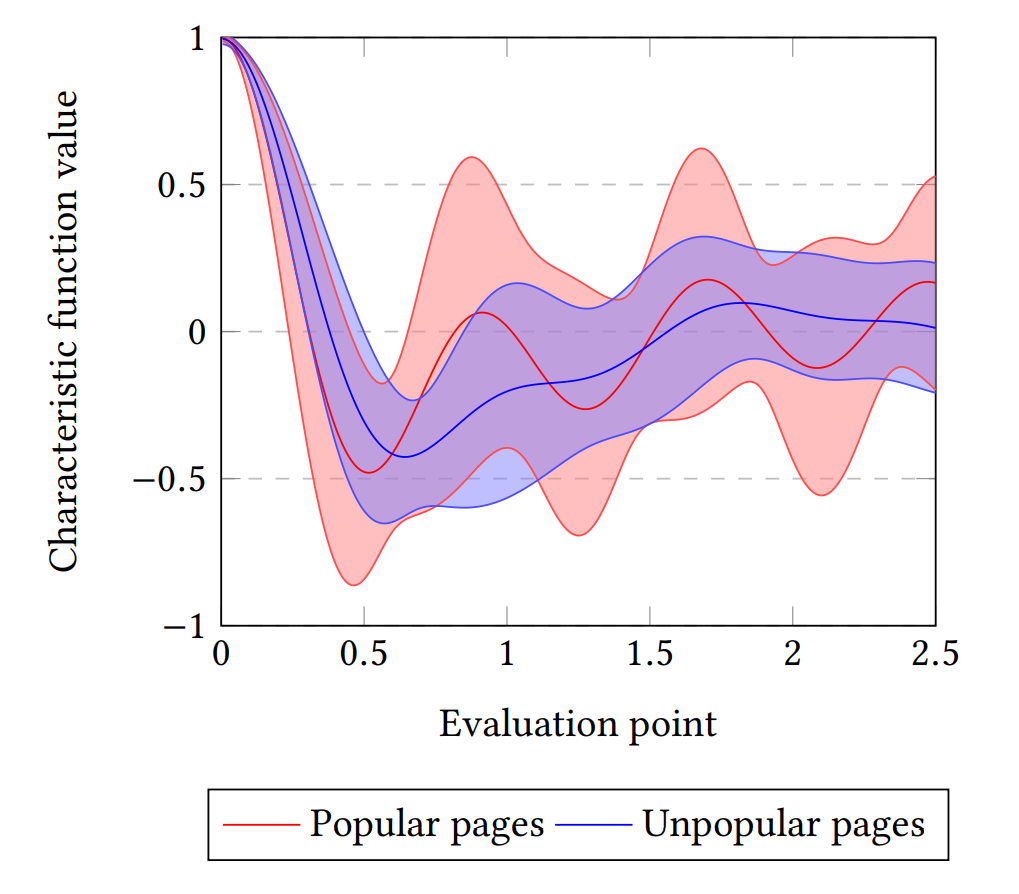
\includegraphics[scale=0.32]{Images/Feather_1.png}
%     \caption{The real part of class dependent mean characteristic functions with standard deviations around the mean for the log transformed degree on the Wikipedia Crocodiles dataset.}
%     % \cite{rozemberczki2020characteristic}
%     \label{fig:Feather}
% \end{figure}


% \begin{itemize}
%     \item \Roni{Graph Embedding}
%     \item \Roni{Graph Embedding for MAPF AS (MAPFAST)}
%     \item \Roni{Omri's approach}
%     \item \Roni{Image-based encoding: sigordson and MAPFASTER}
% \end{itemize}


% \section{Encoding a MAPF Problem as a Graph}
\section{Method}
\label{scn:Methods}

In this section, we describe our AS method for choosing optimal classical MAPF algorithms called MAPF Algorithm selection via Graph embedding (\mapfgas\ ).
%MAPFGAS. \Roni{Is this an acronym?} \Carmel{yes MAPF Graph Algo Selection, maybe need mention this earlier in Abstract}
% MAPFGAS works as follows. \Omri{The acronym used in Abstract is MAG, right?}
% \Roni{I changed the acronym to be MAPF Algorithm selection via Graph embedding (MAG).}
\mapfgas\ works as follows.
First, it encodes the given MAPF problem as a graph.
Then, it creates an embedding of the resulting graph with FEATHER.
The resulting vector is added to a set of previously proposed MAPF-specific features extracted from the given MAPF problem,
and used to solve our AS problem using supervised machine learning.
Next, we describe each of these steps in more detail.


\subsection{Encoding MAPF as a Graph}

We consider two ways to encode a MAPF problem $\Pi=\tuple{k,G,s,t}$ as a graph.
The first encoding method, called \gtv\ , was previously proposed by Ren et al.~\cite{ren2021mapfast}.
\gtv\ encodes $\Pi$ by extracting from $G$ that induced subgraph that includes only nodes that are on a shortest path between the source and the target of an agent.
In more detail, G2V computes for each agent the shortest path from its source to its target while ignoring all other agents.
Then, we construct a graph that contains only the nodes on these shortest paths, adding an edge between any pair of nodes on these shortest paths that have an edge between them in the original MAPF problem.
%\Carmel{<- I changed this} RONI: GOOD, TNX. %and adds to this graph all the nodes and edges that are adjacent to these shortest path nodes. % IS THIS CLEAR? NOT SURE
Note that the resulting graph may be disconnected.

The benefit of G2V is that the resulting graphs are significantly smaller than $G$.
However, these graphs lose information: they do not consider regions on $G$ that are not on the agents shortest paths.
These regions may be important to consider when the corresponding MAPF problem is particularly difficult and agents must move away from their shortest paths.
To address this limitation of \gtv, we propose \emph{FullG2V} (\fgtv\ ), which uses the entire graph $G$ to encode the given MAPF problem.
To include details about the MAPF problem beyond $G$, the graph outputted by \fgtv\ includes an artificial edge for every agent between its source and target.
Formally, for a MAPF problem $\tuple{k,G=(V,E),s,t}$ \fgtv\ outputs the graph $G'=(V',E')$ where
$V'=V$ and $E'=E\cup \{(s(i),t(i))\}_{i=1}^k$. Figure~\ref{fig:graph-encodings} illustrates \gtv\ and \fgtv\ on a simple MAPF problem on a 4-neighborhood grid.
%will \Carmel{'will' is not resulting in result} output a FIXED
%\Roni{Would be nice to show an example of \gtv\ and \fgtv\ side by side} \Carmel{it is shown in Method Flow figure}\Roni{I want a better version. Adding it now.}

\begin{figure}
    \centering
    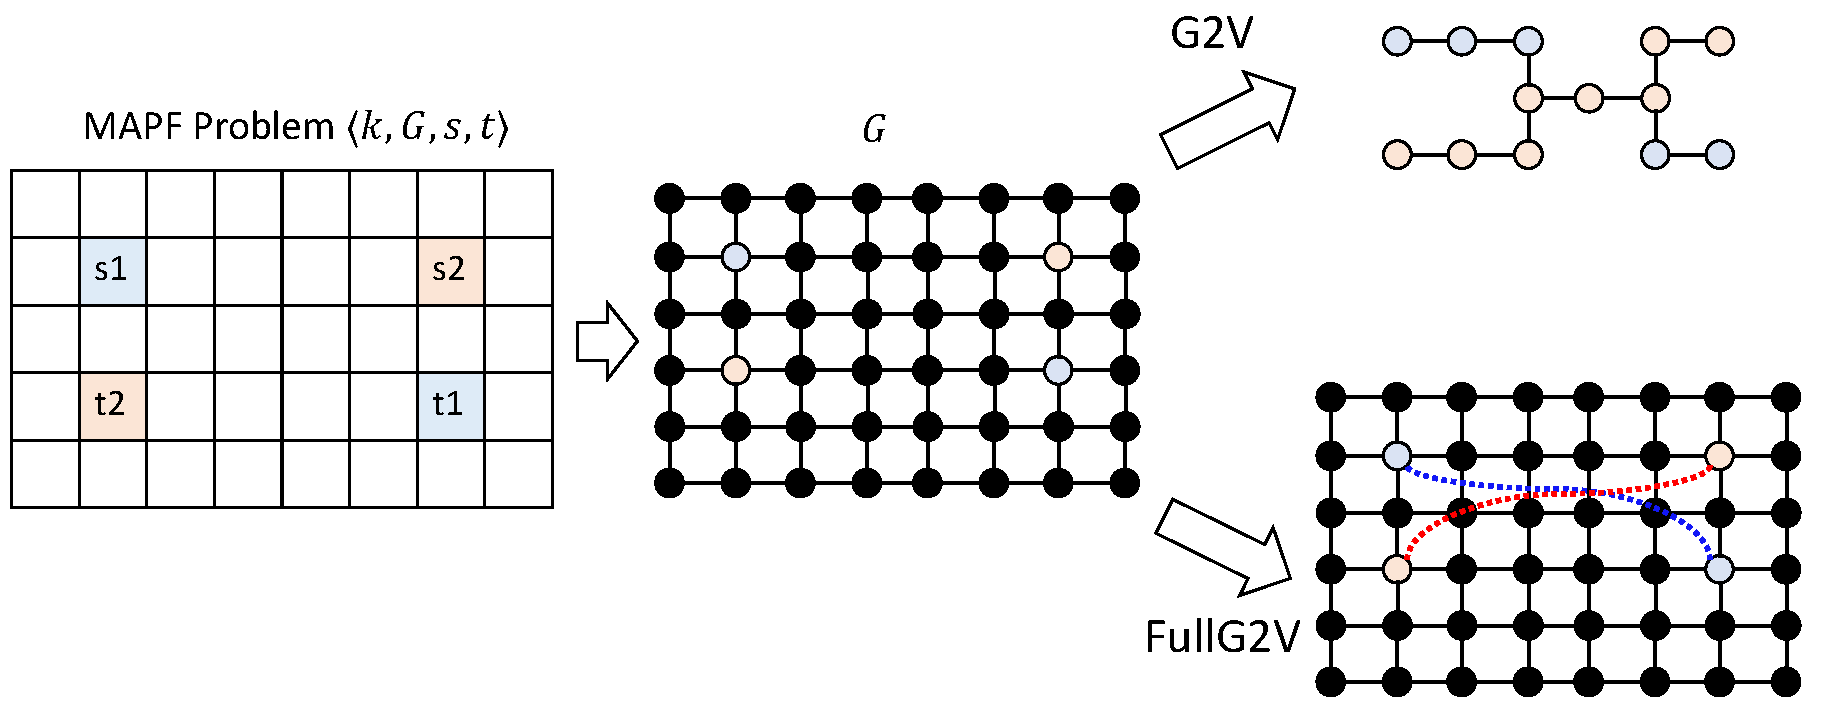
\includegraphics[width=\columnwidth]{Images/MAG-Diagram.pdf}
    \caption{An example of the \gtv\ and \fgtv\ encoding methods. \Carmel{G2V picture is wrong, we dont add nodes outside the shortest paths only add links if any, see my original picture... + it
joins these paths to a single graph and adds links if any between adja-
cent path’s nodes in original MAPF problem}}
    \label{fig:graph-encodings}
\end{figure}


% Spea MAPF problem by taking the entire graph $G$, and adding an artificial edge between every
% $(s_i, t_i)$

% encodes the entire The second way to encode a MAPF problem as a graph t

% In the first phase, we perform novel proposed structural abstraction for each MAPF problem \textbf{we cast a MAPF problem to its Graph representation and add artificial links between each agent's start and goal nodes we called FullG2V}. Another structural abstraction proposed by \cite{ren2021mapfast} called G2V was performed where casting a MAPF problem to its graph representation while using single-agent shortest paths.






% already in that graph.
% Then, it joints
% Each of these
% The results paths are augmented by
% In G2V, the shortest path to reach the goal is computed for each agent while ignoring all other agents.
% The result
% G2V

% ....
% In the first phase, we perform novel proposed structural abstraction for each MAPF problem \textbf{we cast a MAPF problem to its Graph representation and add artificial links between each agent's start and goal nodes we called FullG2V}. Another structural abstraction proposed by \cite{ren2021mapfast} called G2V was performed where casting a MAPF problem to its graph representation while using single-agent shortest paths.

\subsection{Embedding the Graph}

To embed the encoded graph into a vector space, we used the FEATHER algorithm~\cite{rozemberczki2020characteristic}.
FEATHER creates a graph embedding by first embedding each of the graph nodes and then pooling the resulting vectors to a single vector of size 500.
%\Roni{Carmel, can you say more here. How is this pooling done? For example, what is the size of the resulting vector? is it just a parameter? something else? how did you set it?} \Carmel{the resulting vector is 500 length and the polling meathod is hyper parameter of model init - the default is 'mean', we use 'max'}\Roni{But is the 500 a hyper parameter as well or a builtin number in the method?} \Carmel{500 is constant, we can not change it}
Unlike other graph embedding techniques, it does not require a-priori training.
Consequently, the features extracted using FEATHER can be extracted and used in a meaningful way even for graphs created for MAPF problems that are not in the training set.
This is key to allowing graph embedding features to be used for optimal MAPF AS methods.

Note that the default pooling method in FEATHER is ``mean''.
This means the graph embedding is created by taking the mean over its constituent node embeddings.
%\Roni{@Carmel: please verify this} \Carmel{correct}
We observed that using mean pooling did not perform well in our context, i.e., led to poor classification results when used as features.
The reason for this is that mean pooling diminishes the impact of the artificial edges added between the source and target of each agent. Thus, MAPF problems on the same graph yielded very similar embeddings.
To overcome this, we configured FEATHER to use ``max'' pooling, which emphasizes small differences between graphs created from MAPF problems on the same grid. This yielded significantly better results when  training the AS classification model.


%  the only deference related to FullG2V abstractions between graphs obtained from the same grid MAPF problems is the special artificial links between agents location. Basically there is very little difference between graphs from same grid, by max pooling we emphasize the differences between graphs embeddings which works better for training a classification model. \Roni{Excellent explanation}

% is 'mean' resulting in much poor results, this is logical since node level features are pooled by the pooling method to create graph level statistics, and the only deference related to FullG2V abstractions between graphs obtained from the same grid MAPF problems is the special artificial links between agents location. Basically there is very little difference between graphs from same grid, by max pooling we emphasize the differences between graphs embeddings which works better for training a classification model. \Roni{Excellent explanation}


% Using FEATHER allows us to

% The main advantage of FEATHER over prior work on gr
% Given the graph encoding of

% To embed the resulting graph into a vector space, we used the FEATHER algorithm~\cite{rozemberczki2020characteristic}.
% Different from the default implementation of FEATHER, we set the pooling here to ....\Roni{Carmel can you plug here your use of max pooling and th motivation}


% For structural abstraction shown we have used \href{https://github.com/benedekrozemberczki/karateclub/tree/master/karateclub/graph_embedding/}{Feather Graph embedding model} provided by the  Benedek et al. \cite{rozemberczki2020characteristic}, with the following non default hyper parameters: pooling='max'. The default value of 'pooling' is 'mean' resulting in much poor results, this is logical since node level features are pooled by the pooling method to create graph level statistics, and the only deference related to FullG2V abstractions between graphs obtained from the same grid MAPF problems is the special artificial links between agents location. Basically there is very little difference between graphs from same grid, by max pooling we emphasize the differences between graphs embeddings which works better for training a classification model. \Roni{Excellent explanation}



\subsection{Feature Extraction and Learning}
% ...something about how we combinted the features and something about the  learning
% In the first phase, we perform novel proposed structural abstraction for each MAPF problem \textbf{we cast a MAPF problem to its Graph representation and add artificial links between each agent's start and goal nodes we called FullG2V}. Another structural abstraction proposed by \cite{ren2021mapfast} called G2V was performed where casting a MAPF problem to its graph representation while using single-agent shortest paths.

% In the second phase, independently for each graph abstraction explained above we use Feather algorithm from karateclub\footnote{ \url{https://github.com/benedekrozemberczki/karateclub/tree/master/karateclub/graph_embedding/}}
% %\href{https://github.com/benedekrozemberczki/karateclub/tree/master/karateclub/graph_embedding/}{Feather implementation from karateclub}
% provided by Benedek et al. \cite{rozemberczki2020characteristic} presented in section \ref{scn:Feather}, to train it with graphs  obtained from the train set. \Carmel{This is wrong its not unsupervised training, Roni can you fix please?} Training this model means preforming an unsupervised learning for the train MAPF problems graphs representations. The trained resulting models are used to get all graphs embeddings which is used later for training and testing a Machine Learning (ML) model. \Omri{Last sentence needs rephrasing - if not sure how to rephrase let us do this together}

For a given MAPF problem $\Pi$, \mapfgas\ uses \gtv\ and \fgtv\ to create two graphs $G_\gtv\ $ and $G_\fgtv\ $ that encoding $\Pi$.
Then, it creates two graph embeddings $v_\gtv\ $ and $v_\fgtv\ $ by applying FEATHER on these graphs.
It also creates a vector $v_\kaduri\ $ by extracting all the MAPF-specific features proposed by Kaduri et al.~\cite{kaduri2020algorithm}.
Finally, \mapfgas\ concatenates
$v_\gtv\ $, $v_\fgtv\ $, and $v_\kaduri\ $.
The resulting vector is the features \mapfgas\ uses for training.
The training process itself is a straightforward multi-class supervised learning process,
where every instance is a MAPF problem instance and the label is the fastest algorithm for that instance within our portfolio of algorithms.
Figure~\ref{fig:mgs-features} illustrates the feature extraction and training process.
Note that more sophisticated approaches to AS exists in other domains~\cite{kerschke2019automated}, e.g., methods that involve runtime predictions. This is left for future work.
% More sophisticated AS approaches also exists in other domains.

% \Roni{TODO: Add references to fancier AS approachs, e.g., thoses used by SAT AS}
% Figure \ref{fig:MAPFASG flow} illustrates the entire \mapfgas\ algorithm.


\begin{figure}
    \centering
    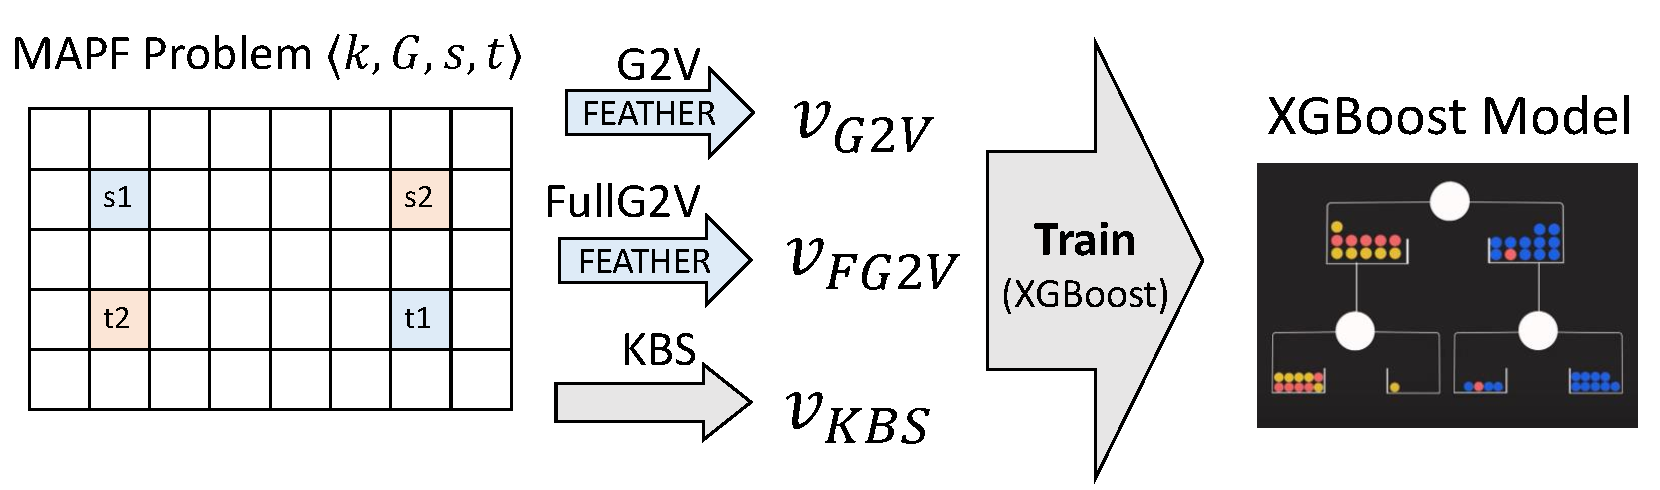
\includegraphics[width=\columnwidth]{Images/MGS-Diagram-New.pdf}
    \caption{Diagram of the \mapfgas\ feature extraction and training process.}
    \label{fig:mgs-features}
\end{figure}
\begin{figure*}
    \centering
    
\includegraphics[width=0.13\textwidth]{Images/empty-16-16.pdf}\enspace
    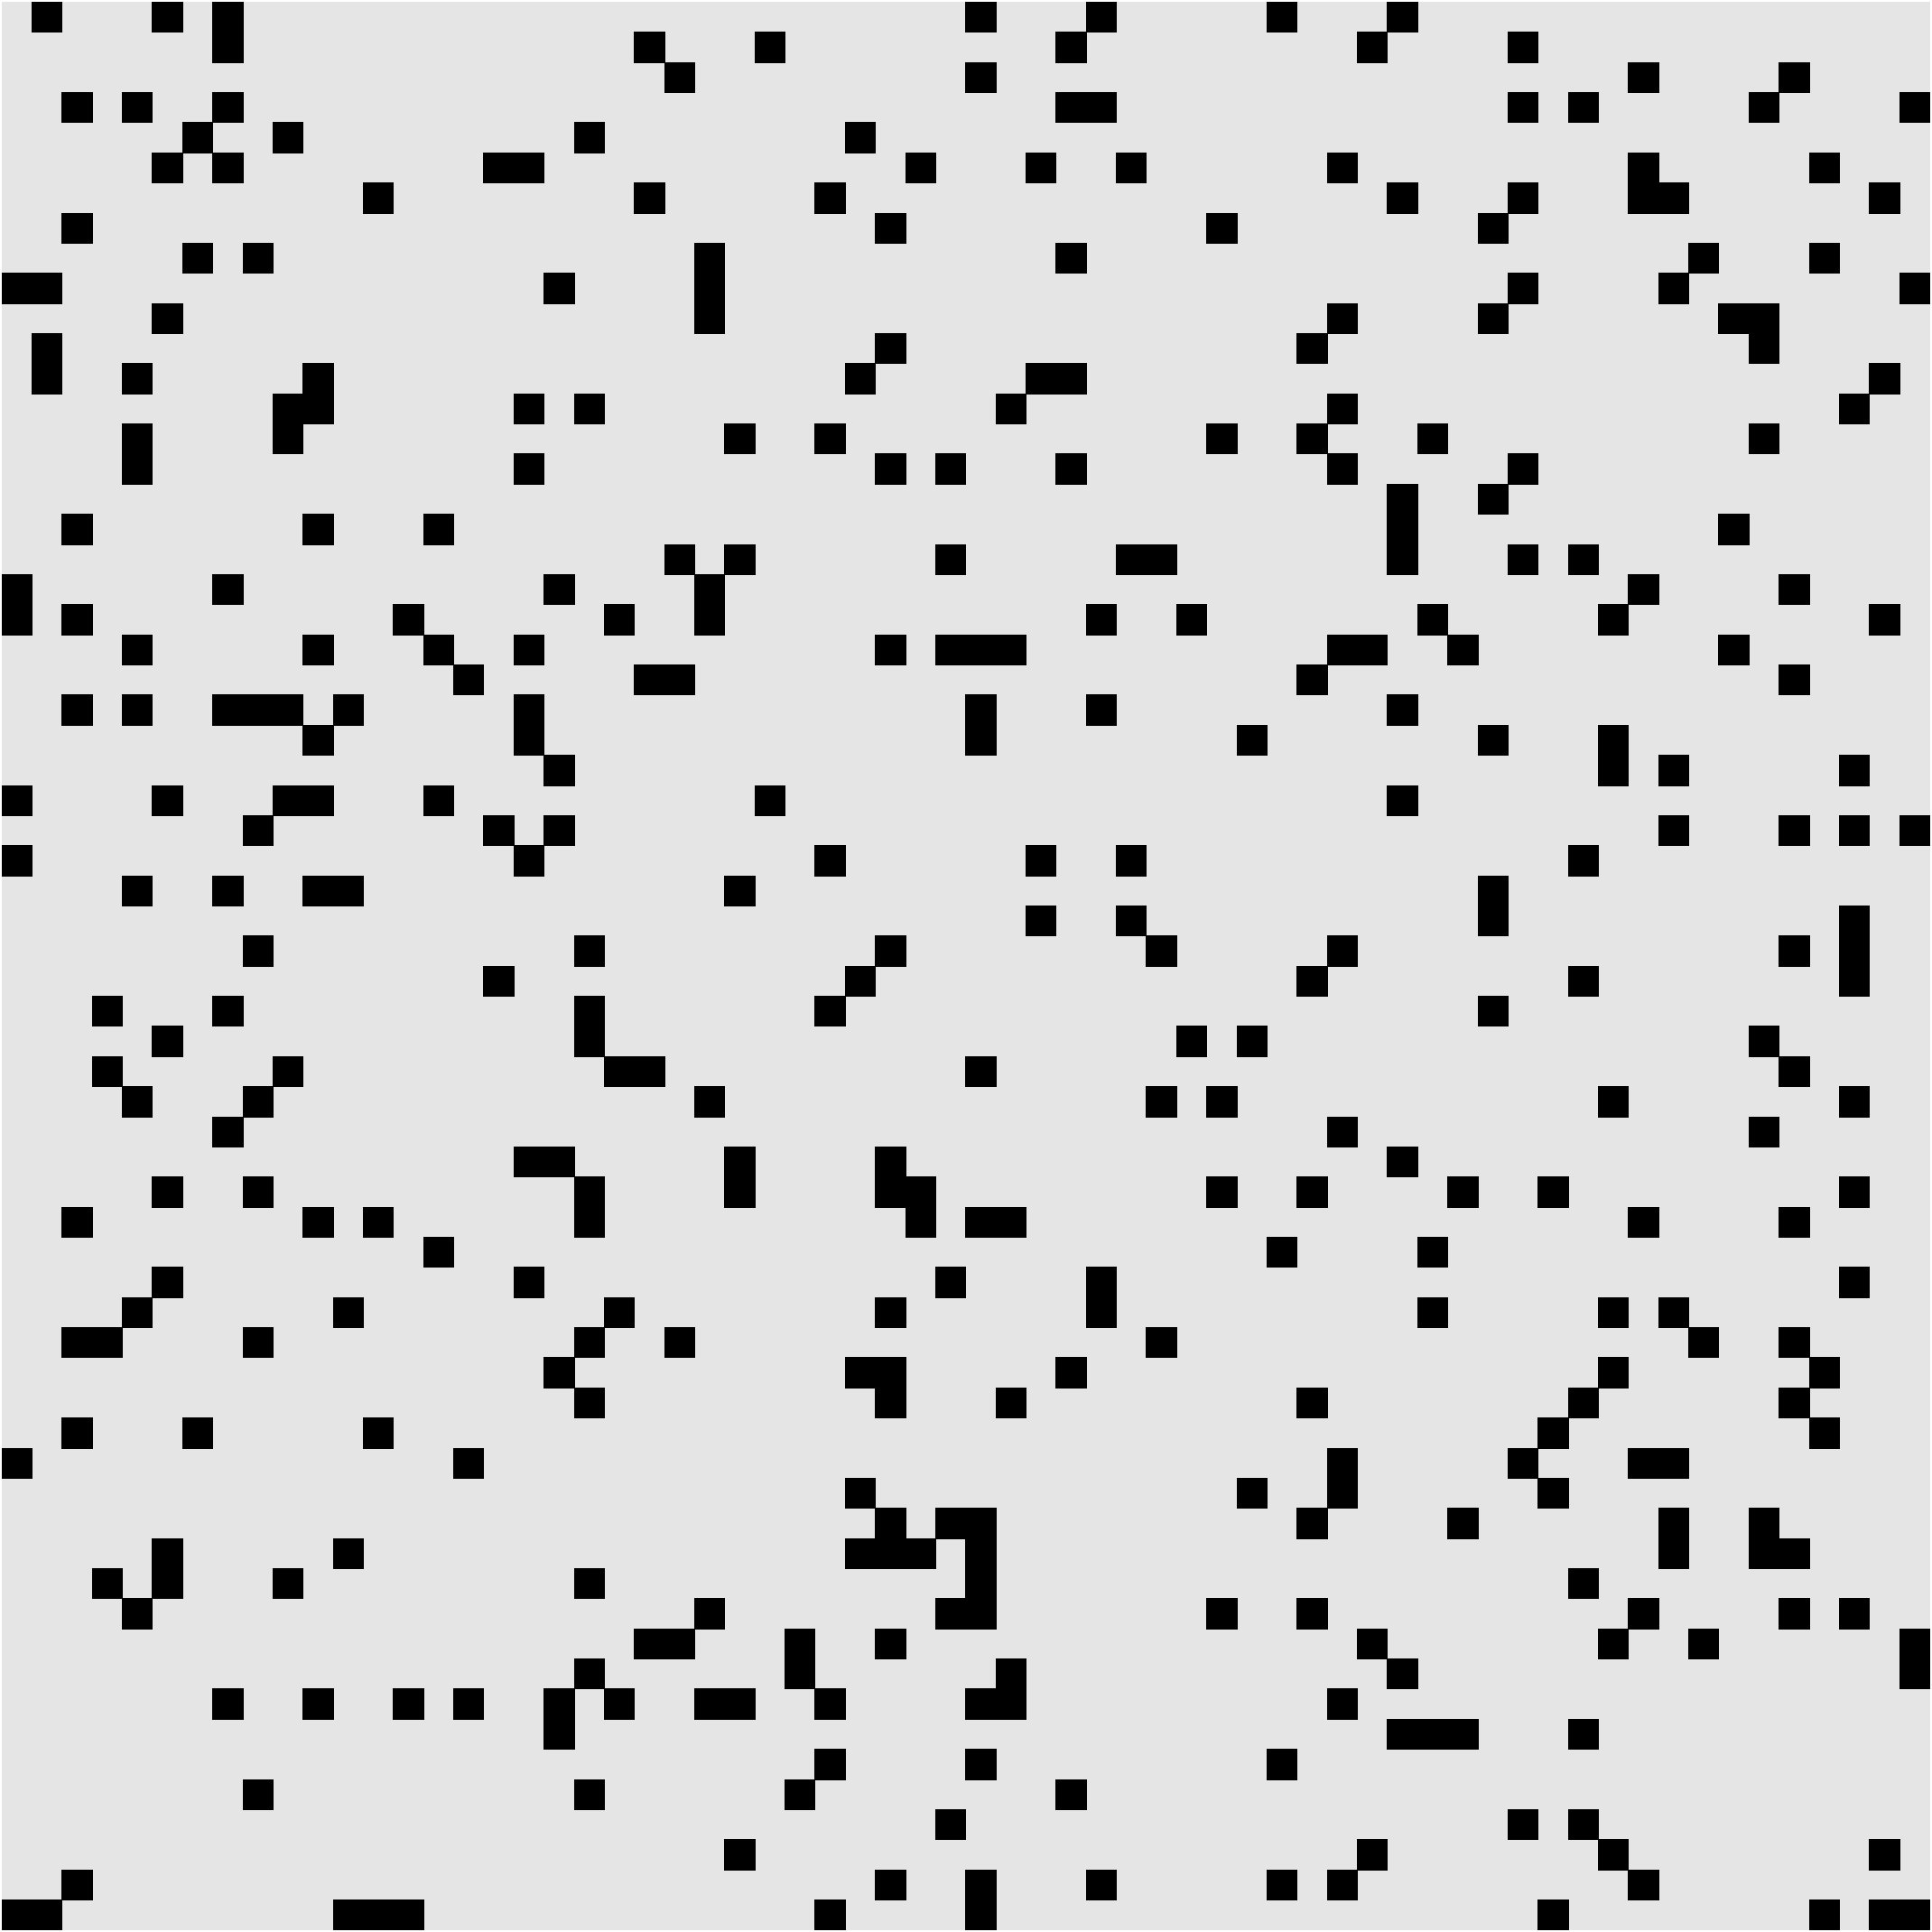
\includegraphics[width=0.13\textwidth]{Images/random-64-64-10.pdf}\enspace
    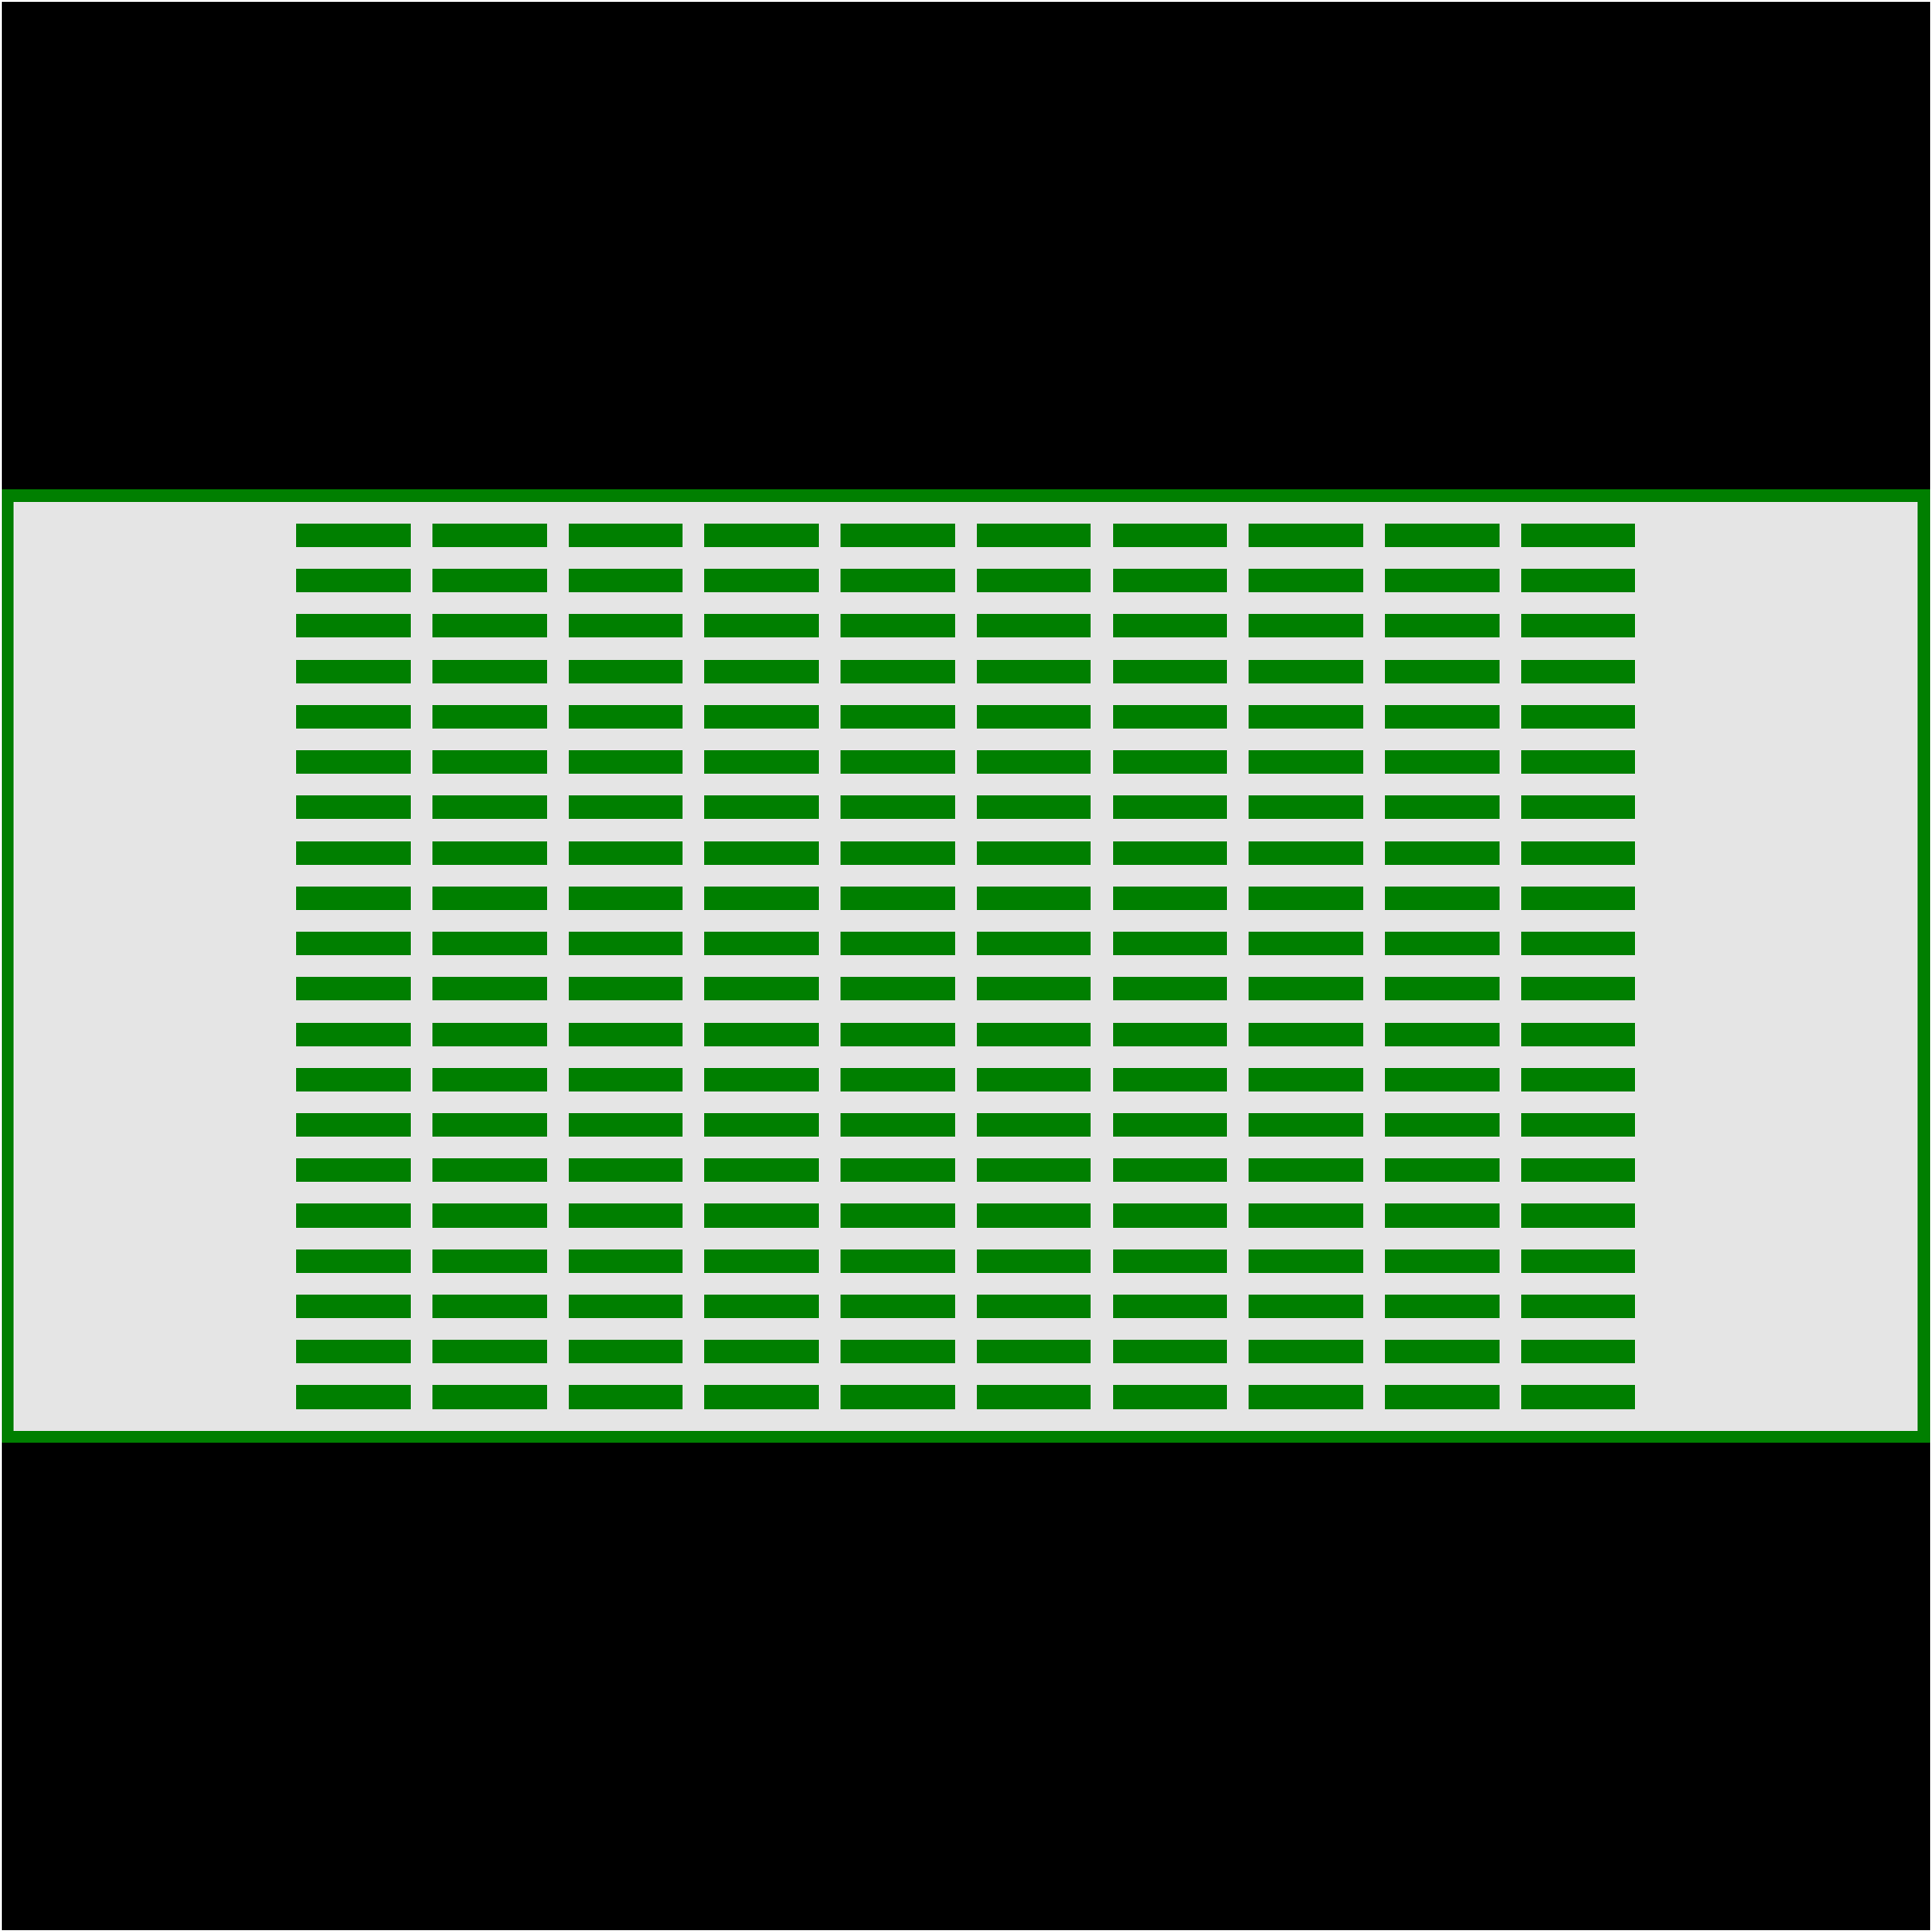
\includegraphics[width=0.13\textwidth]{Images/warehouse-10-20-10-2-2.pdf}\enspace
    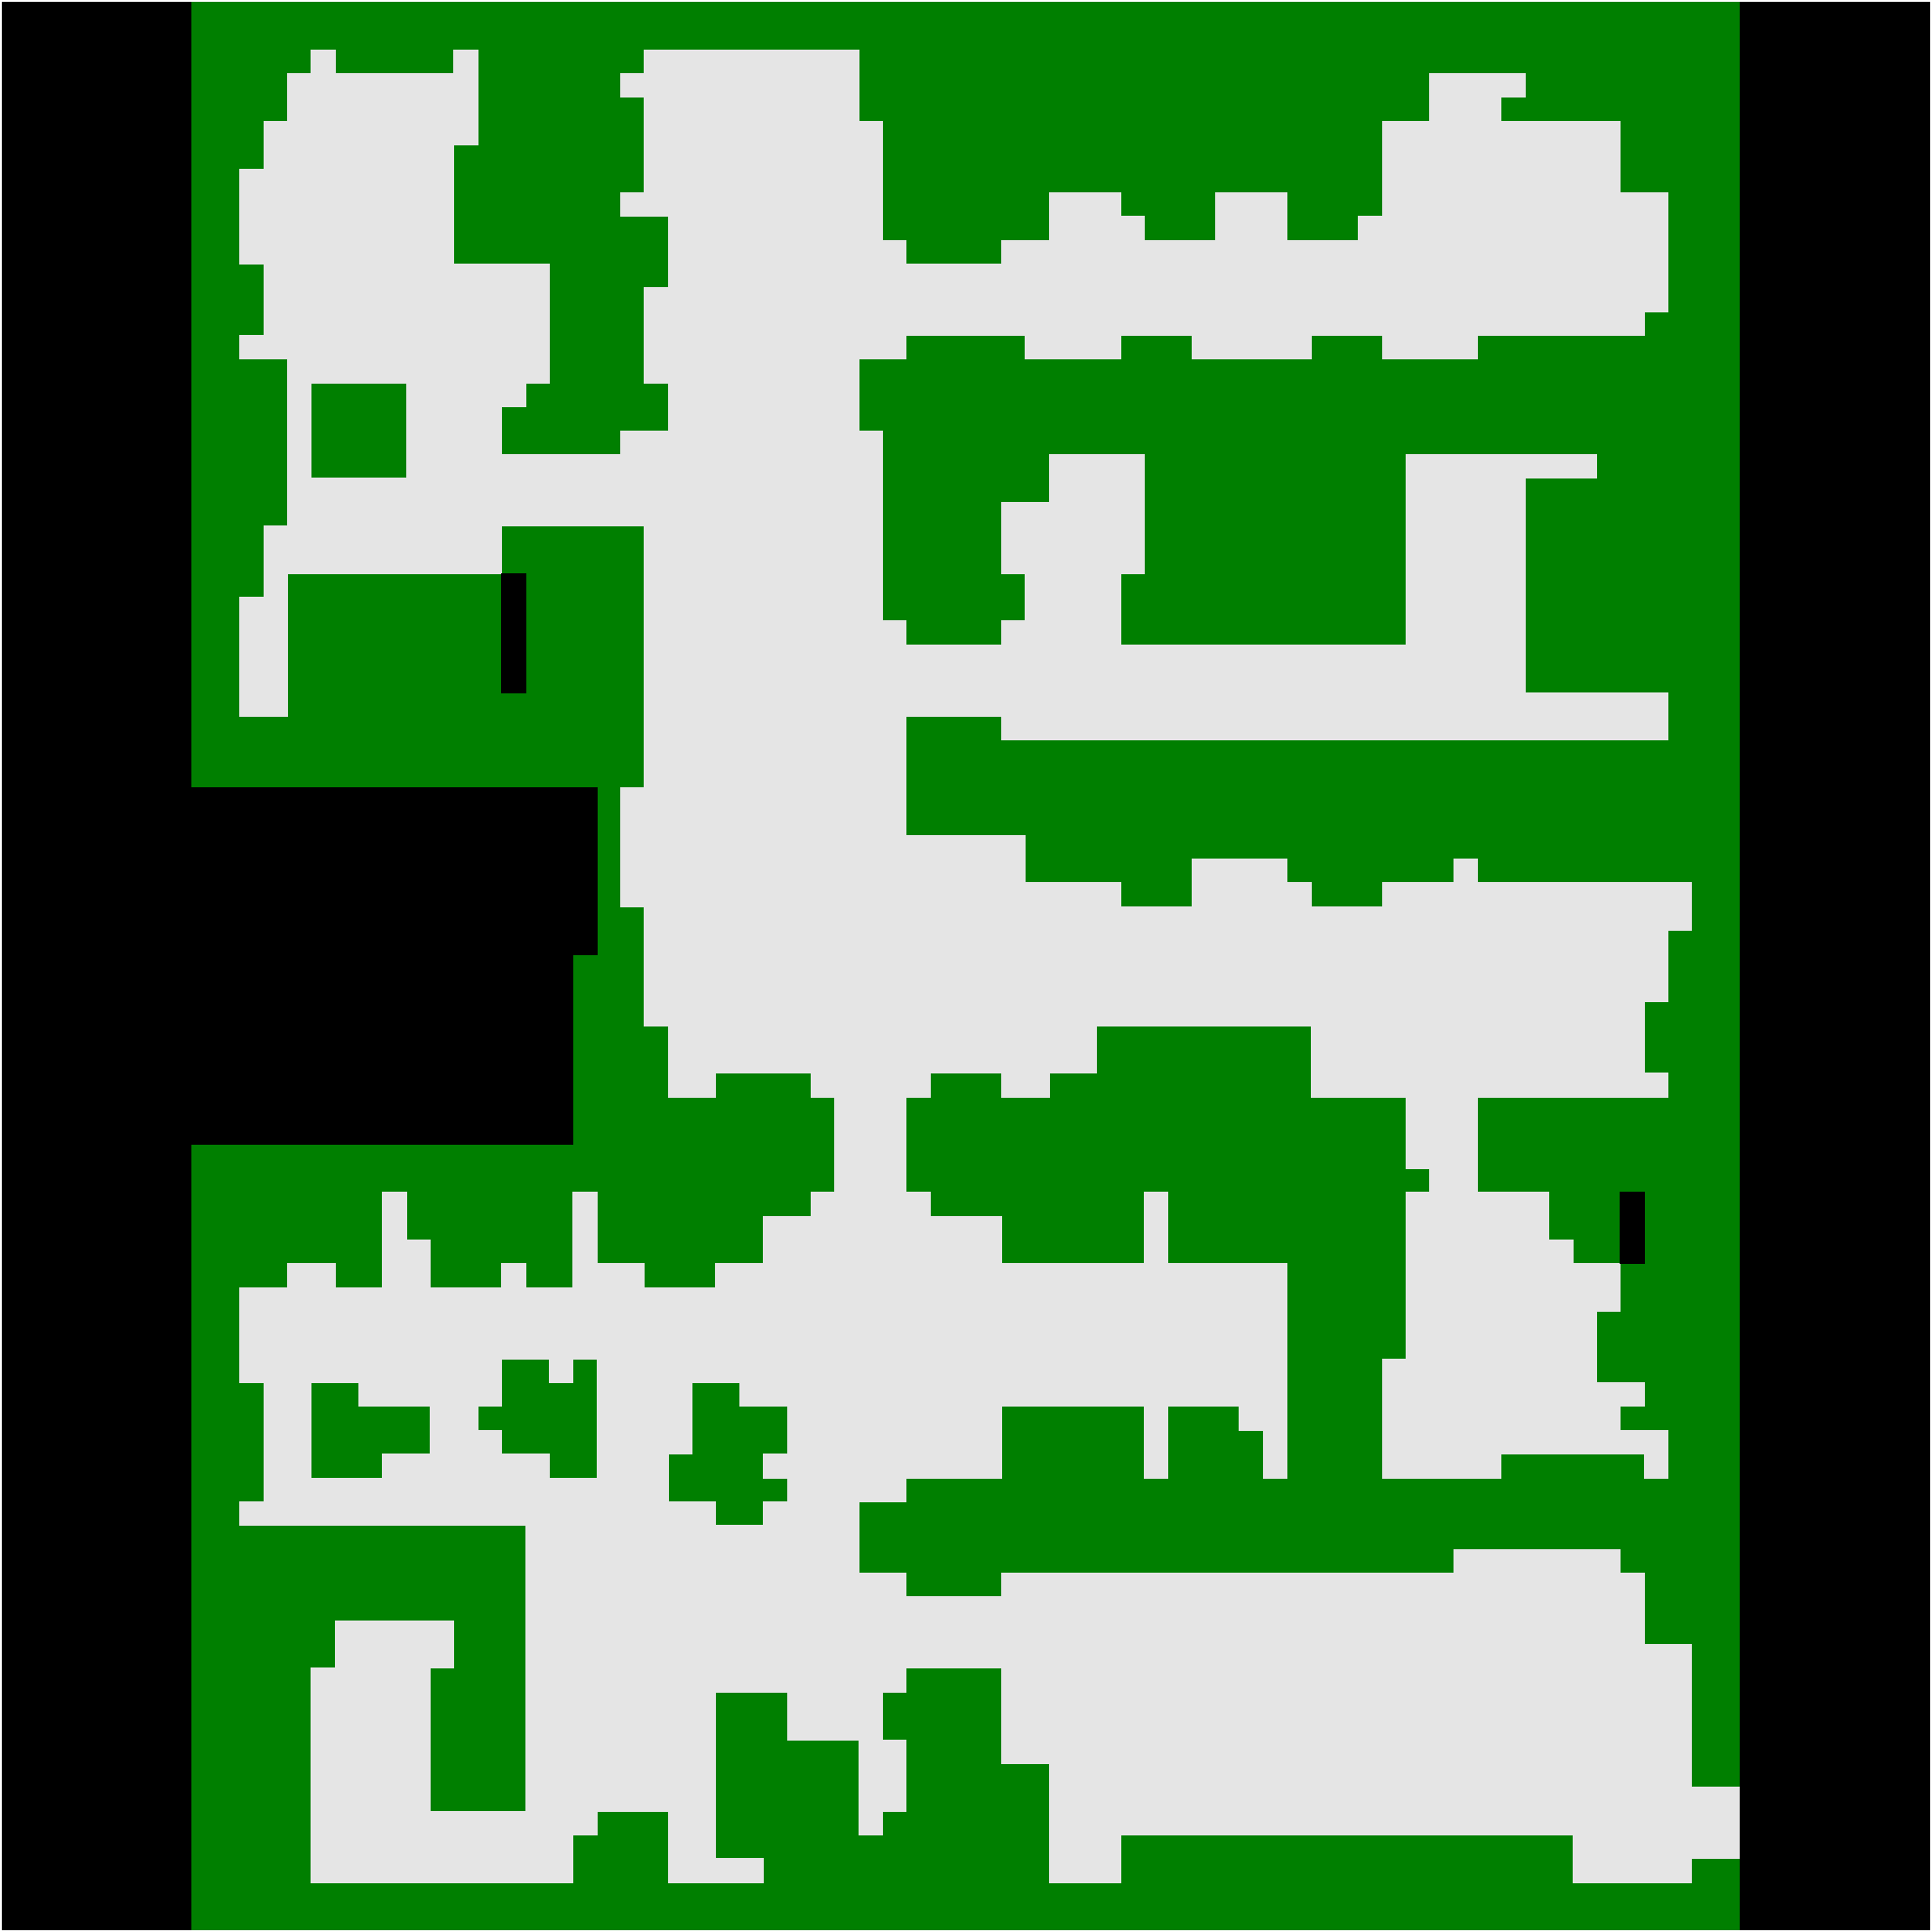
\includegraphics[width=0.13\textwidth]{Images/game-den312d.pdf}\enspace
    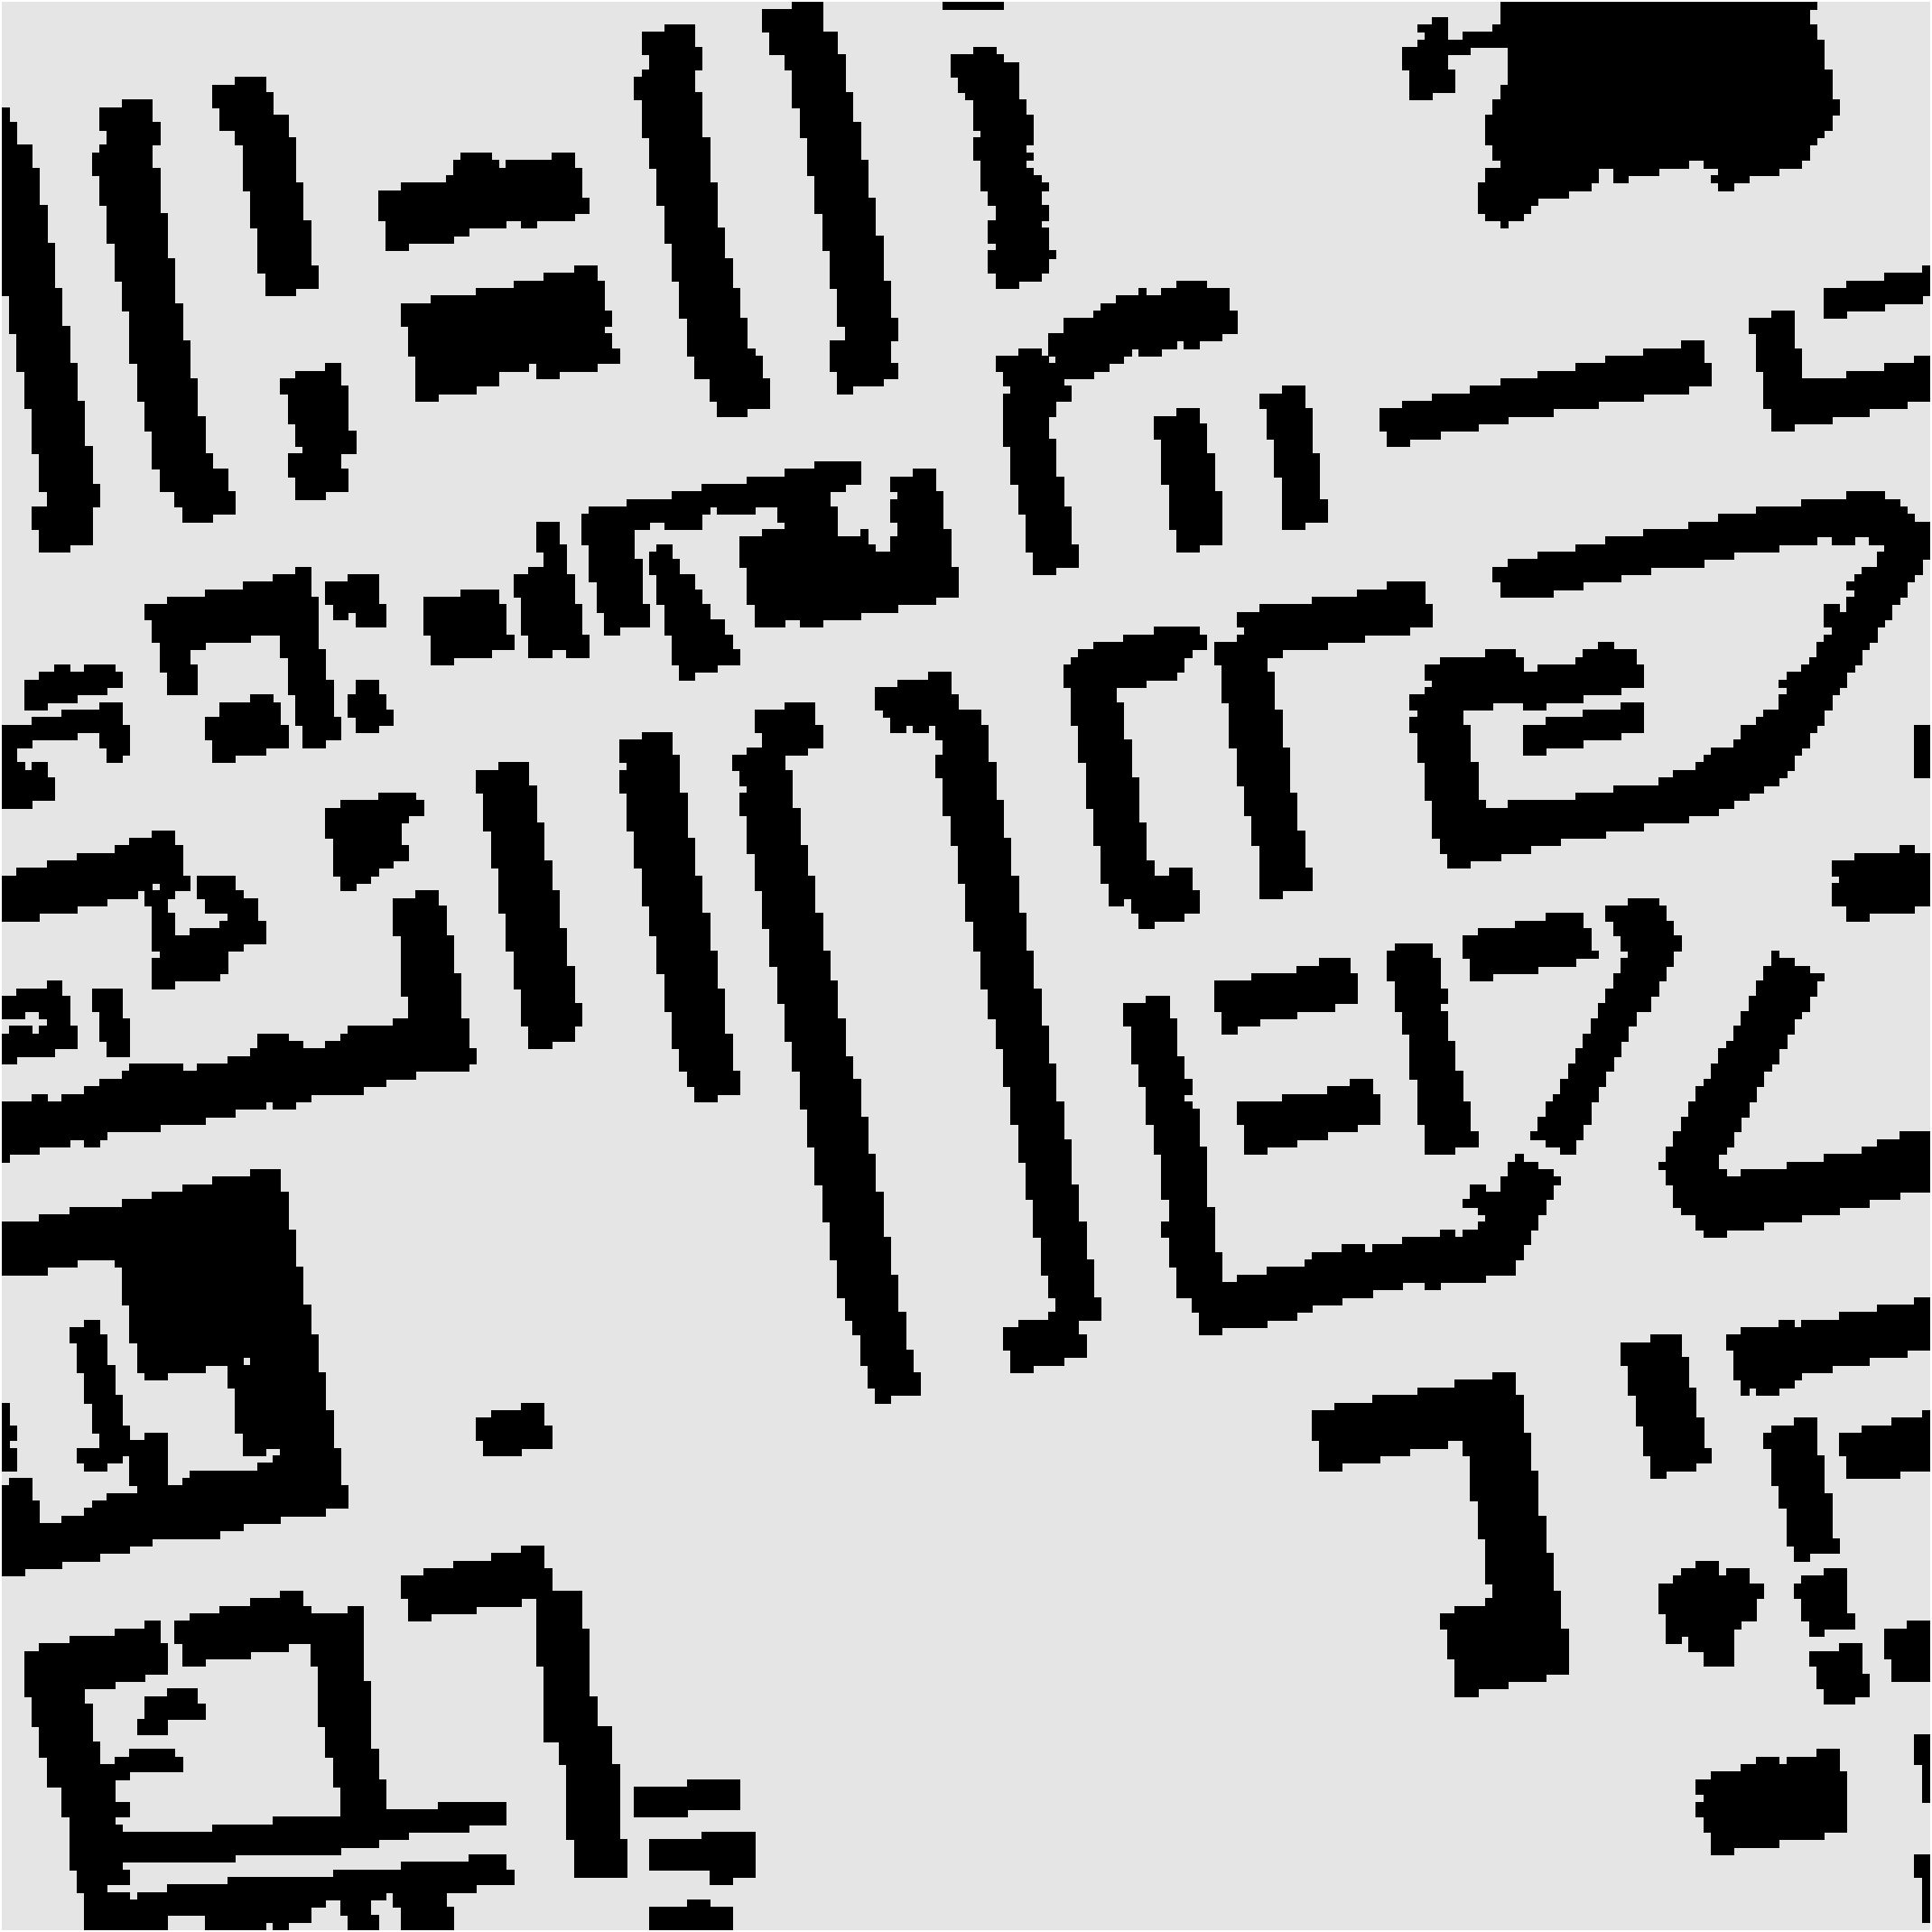
\includegraphics[width=0.13\textwidth]{Images/city-Berlin_1_256.pdf}\enspace
    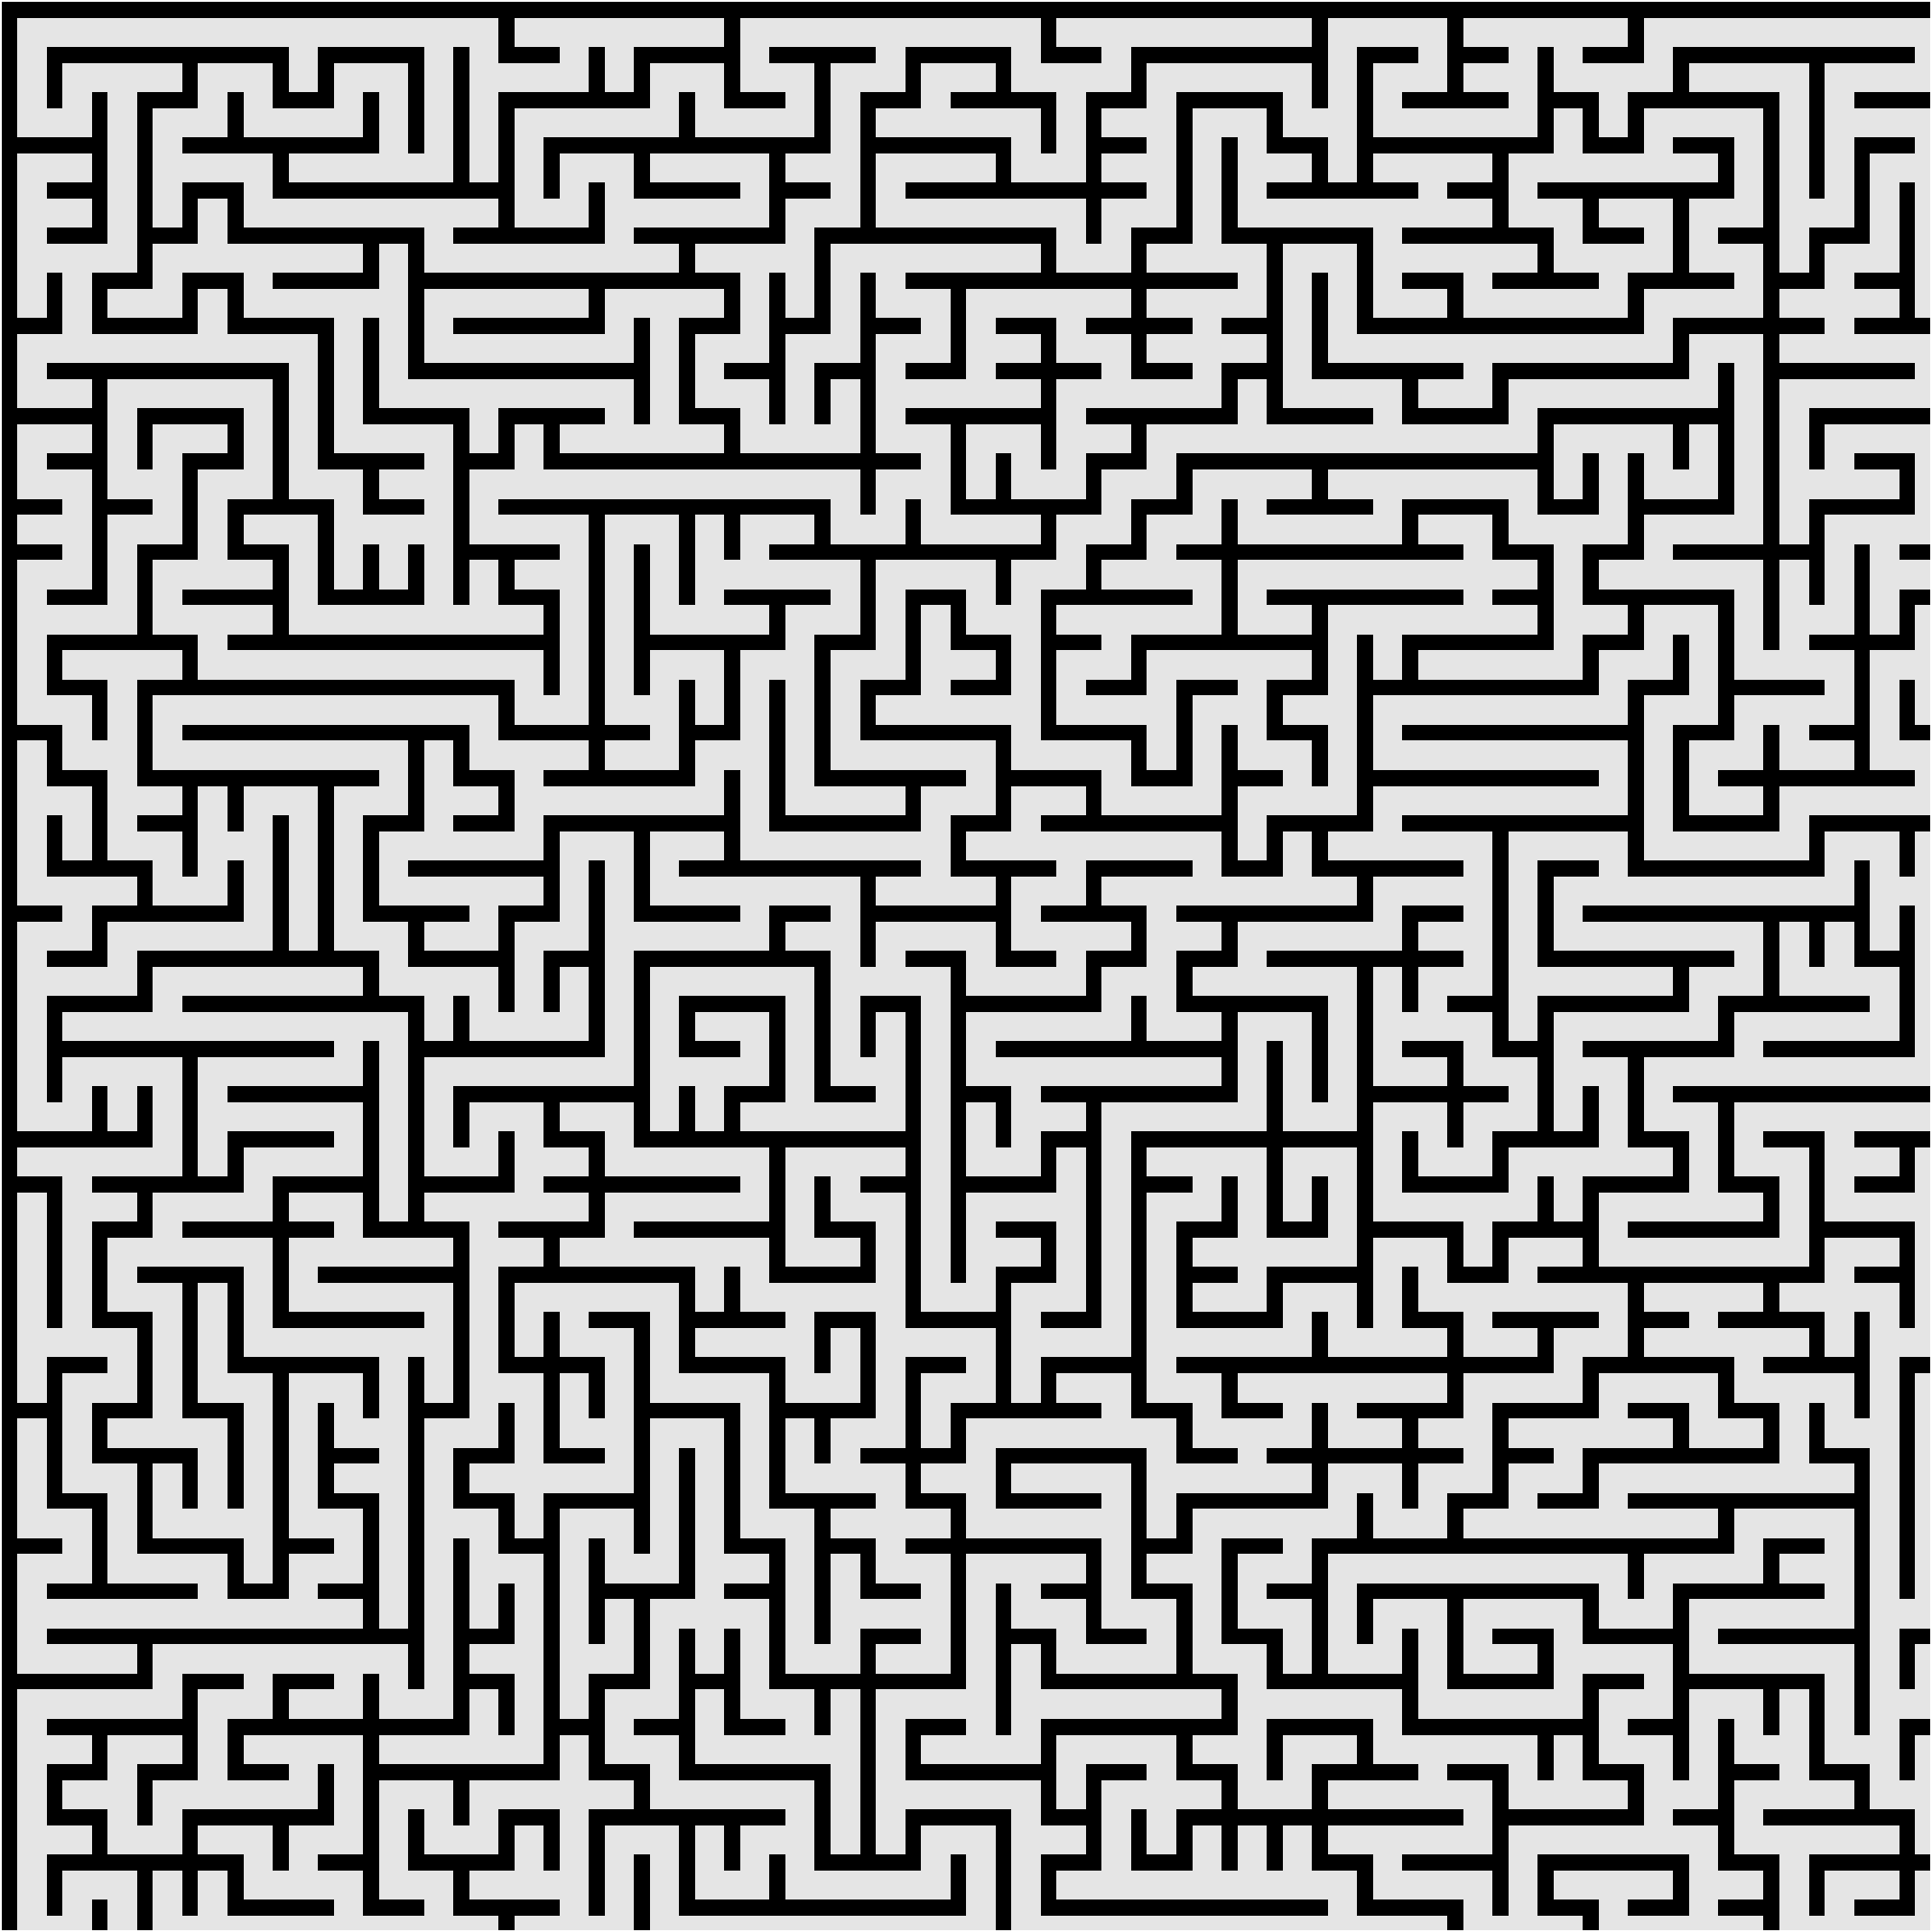
\includegraphics[width=0.13\textwidth]{Images/maze-128-128-2.pdf}\enspace
    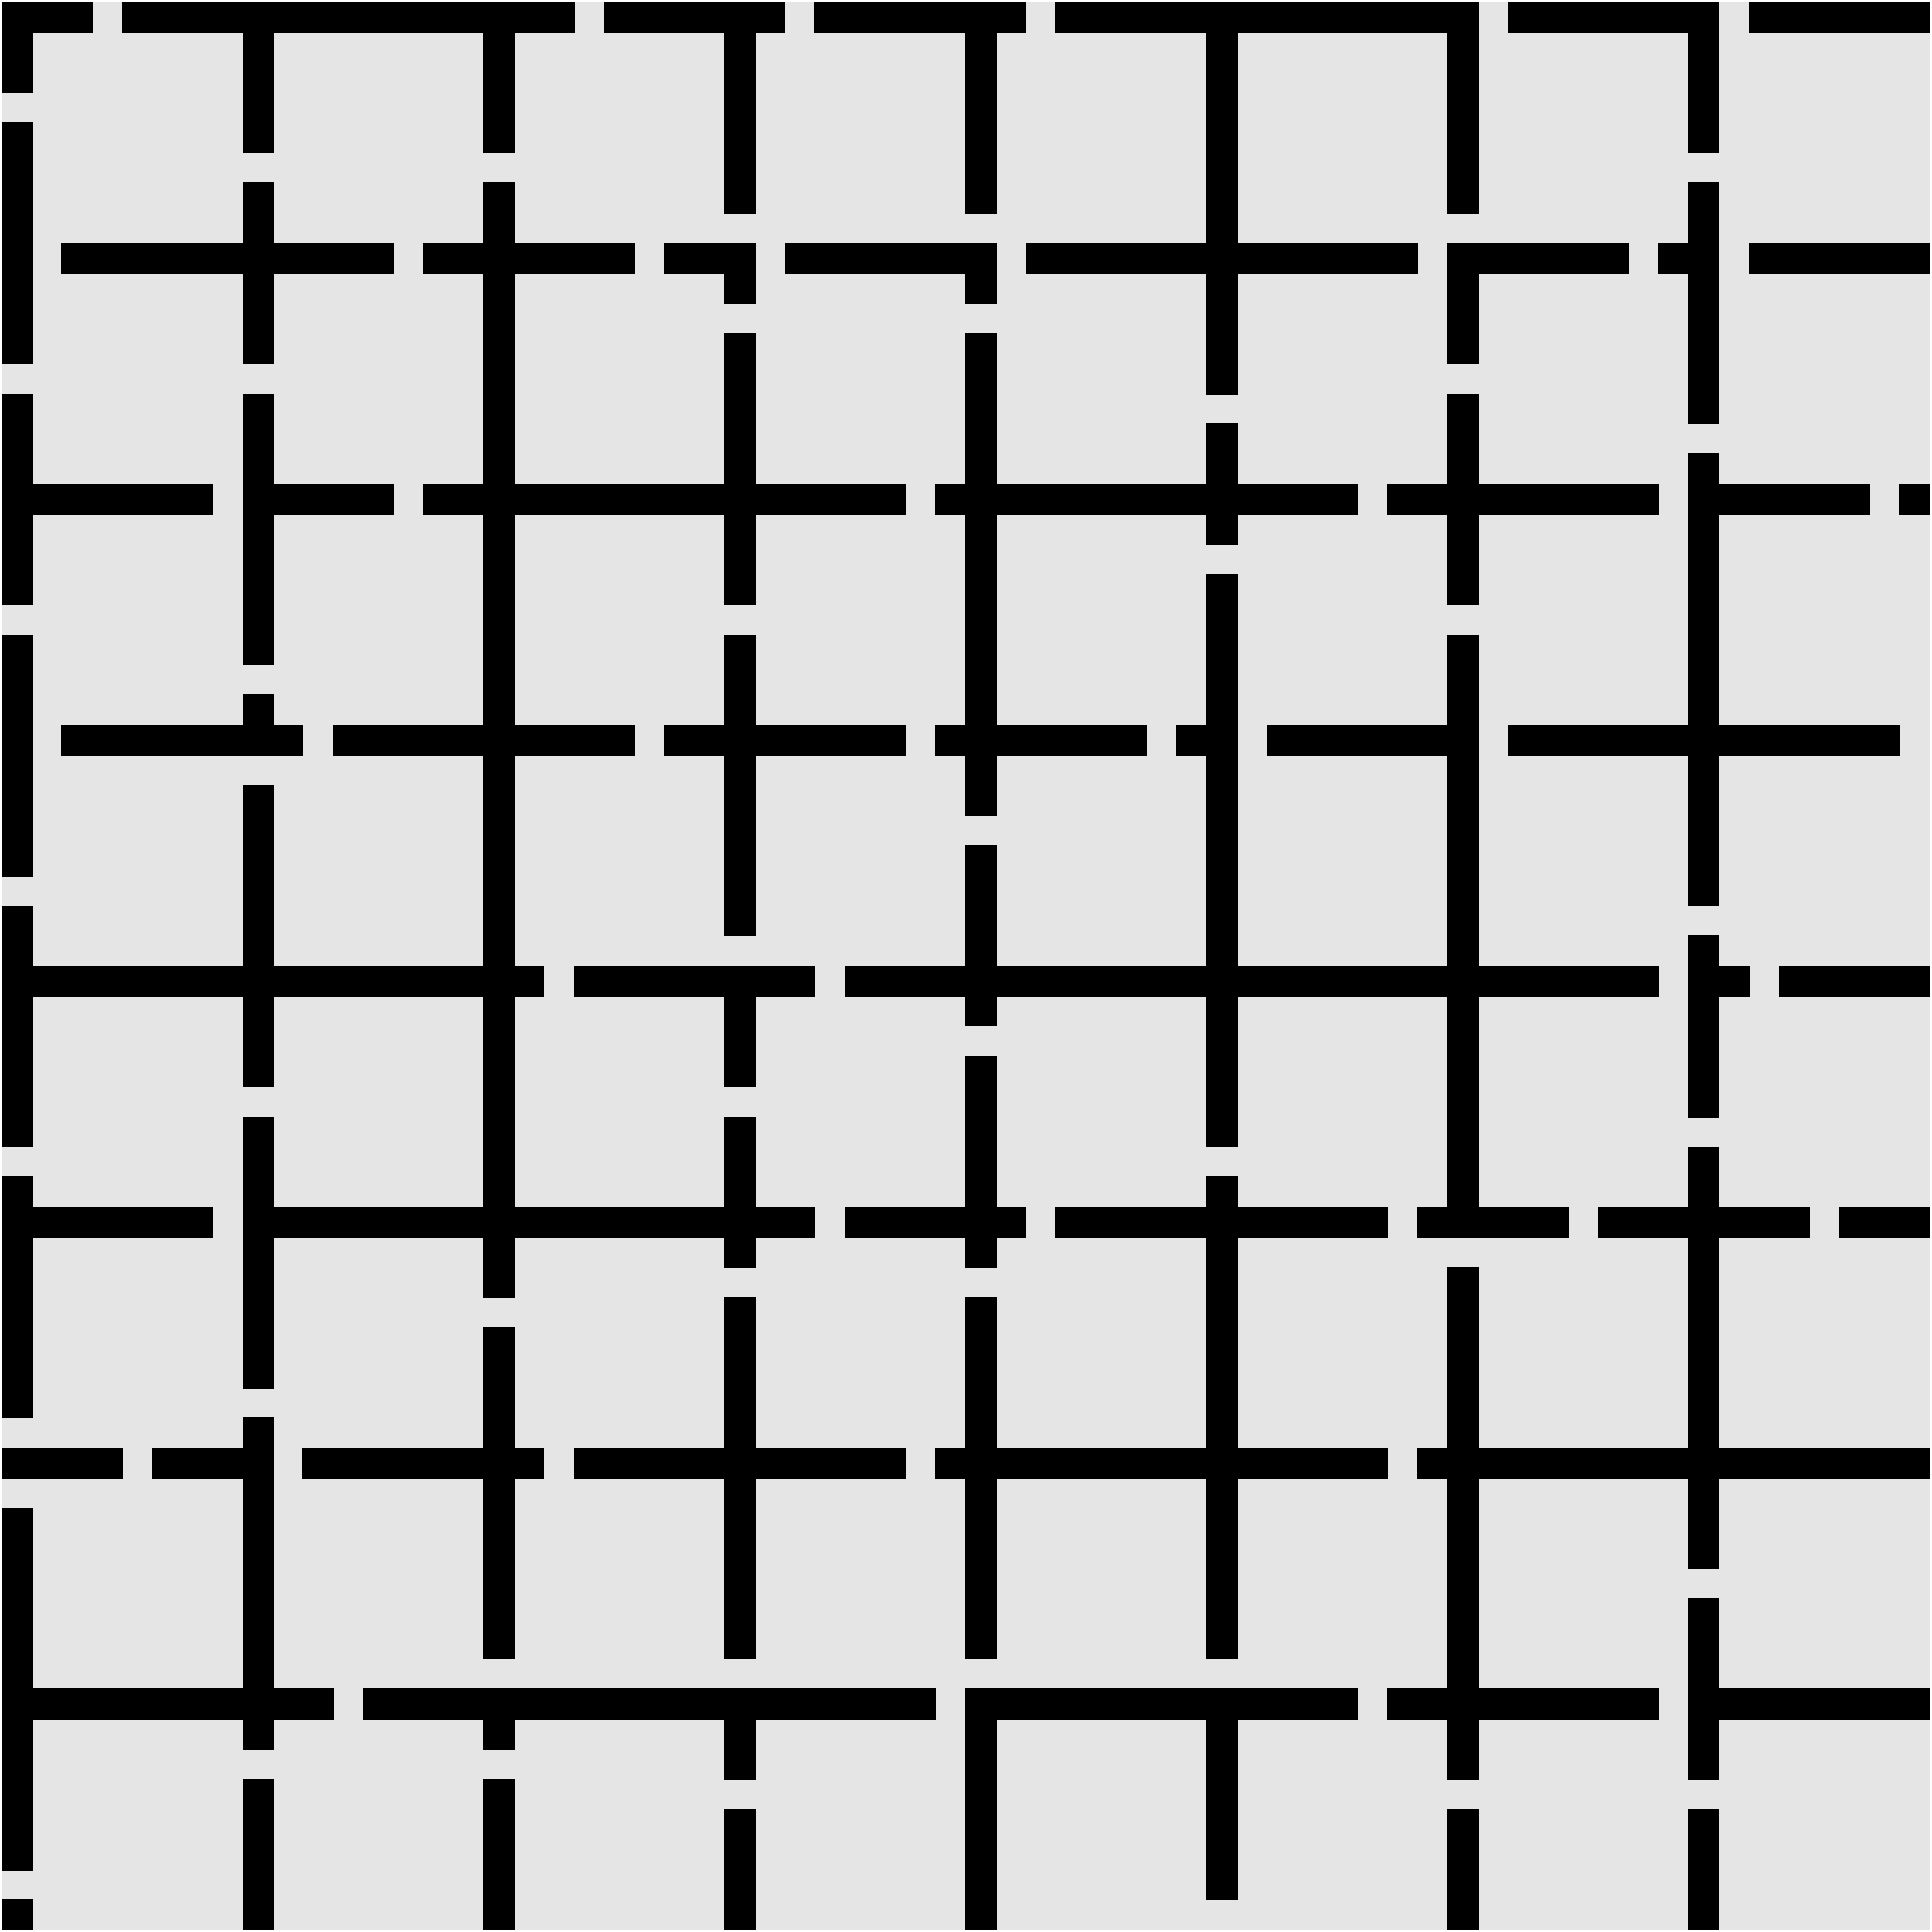
\includegraphics[width=0.13\textwidth]{Images/room-64-64-8.pdf}
    \caption{An example grid from each of the grid types in our benchmark, From left to right: empty, random, warehouse, game, city, maze, and room.}
    \label{fig:grid-types}
\end{figure*}

% classification task.
% These graph embeddings and a vector

% the graph embeddings created by FEATHER for the G2V and FullG2v we create a tensor concatenating both graph embedding and handcrafted embeddings proposed by \cite{kaduri2020algorithm} for training a variety of ML classification models to select the fastest MAPF algorithm. \Carmel{ THIS TO REMOVE: The dataset for classification the models will be constructed for each MAPF problem vector as a concatenation between Graph Embedding and its special handcrafted features presented by Kaduri \cite{kaduri2020algorithm}}. \Omri{Rephrase: Furthermore, we add handcrafted features as done in Kaduri et al. to our models.  }

% The graph embedding
% In the second phase for each MAPF problem, using the graph embeddings obtained both from G2V and FullG2v we create a tensor concatenating both graph embedding and handcrafted embeddings proposed by \cite{kaduri2020algorithm} for training a variety of ML classification models to select the fastest MAPF algorithm. \Carmel{ THIS TO REMOVE: The dataset for classification the models will be constructed for each MAPF problem vector as a concatenation between Graph Embedding and its special handcrafted features presented by Kaduri \cite{kaduri2020algorithm}}. \Omri{Rephrase: Furthermore, we add handcrafted features as done in Kaduri et al. to our models.  }


% \begin{figure}[!h]
%     \centering
%     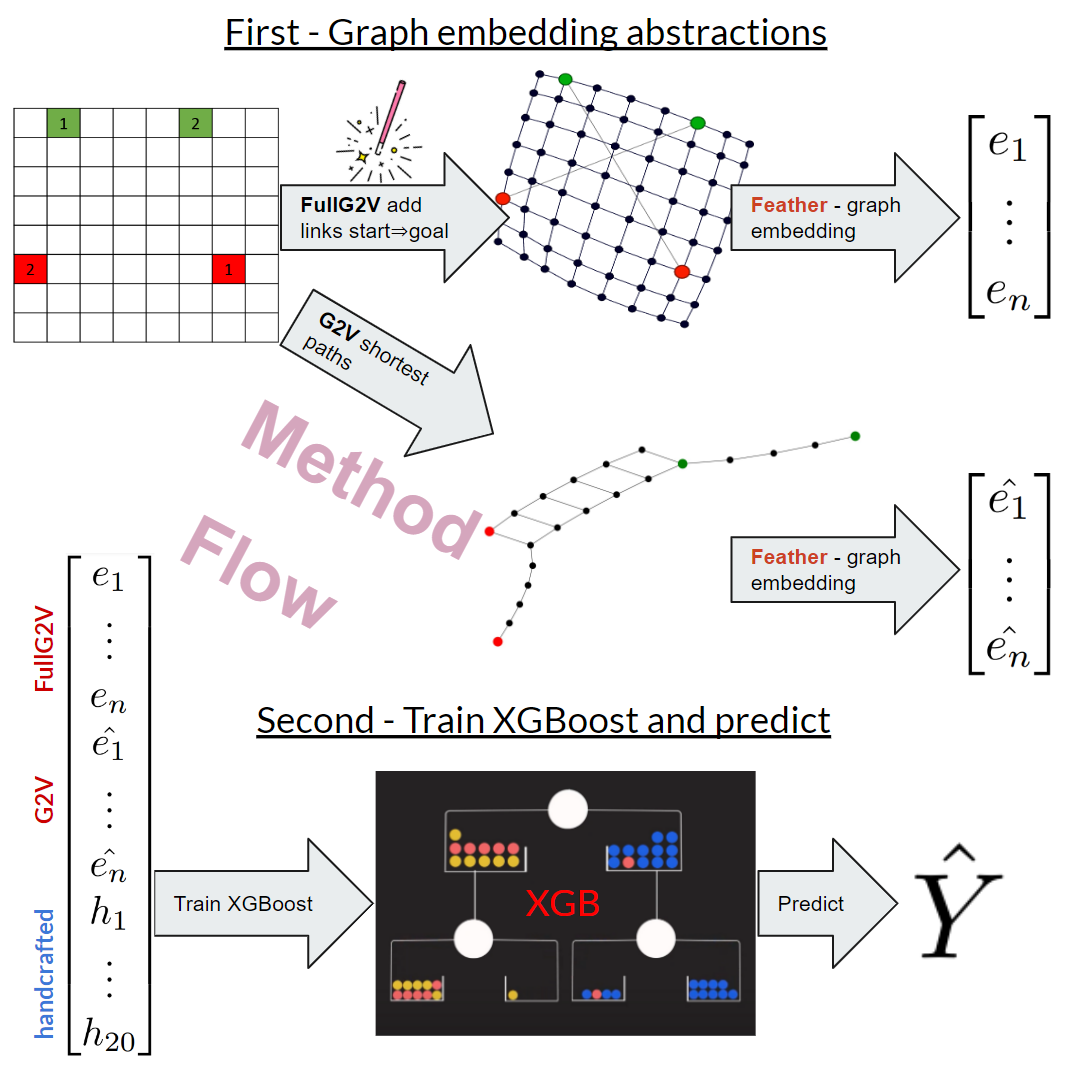
\includegraphics[scale=0.31]{Images/triple_FullG2V_flow.png}
%     \caption{High level design of MAPFGAS}
%     \label{fig:MAPFASG flow}
% \end{figure}

% \section{Problem Definition}
% \label{scn:ProblemDef}
% TBD
% \Omri {I don't think this section is required}

% \section{Research Questions}
% \label{scn:Research}
% \begin{enumerate}
% \item Is it possible to achieve state of the art result for selecting best MAPF search algorithm in benchmark dataset {\cite{kaduri2020algorithm}} using multiple MAPF topological abstraction based approaches such as graph embeddings?
% % \item Is it possible to achieve state of the art accuracy for selecting best MAPF search algorithm in benchmark dataset using Capsules Neural Network based approach {\cite{hinton2018matrix}}
% \end{enumerate}

\section{Experimental Results}
\label{scn:EXPERIMENT}



% \subsection{Dataset} %removedVspace
In this section, we present an experimental evaluation of \mapfgas\ on a standard publicly available grid-based MAPF benchmark~\cite{stern2019multi}.
This benchmark contains 33 grids arranged into seven \emph{grid types}: video
games (denoted as ``game'' grids), city maps (``city''), maze-like
grids (``maze''), grids arranged as rooms with narrow doors
between them (``room''), open grids (``empty''), open grids with
randomly placed obstacles (``random''), and grids that are inspired by the structure of warehouses (``warehouse'').
Figure~\ref{fig:grid-types} shows an example grid from each type.\footnote{The images were taken from the MovingAI repository~\cite{sturtevant2012benchmarks}, which hosts the grid MAPF benchmark we used~\cite{stern2019multi}.}
%\Roni{Would be neat to show a figure with an example from each grid type, to make it more self-contained.}
The benchmark includes \emph{scenario files} for each grid.
Each scenario file contains source and target locations for as many as 1,000 agents.\footnote{Every scenario file contains 1,000 pairs of start and target locations, except for grids that are too small to occupy that many agents.} % where possible.
The scenario files of each grid are grouped into two sets.
In the first set of scenario files, denoted
\emph{Random},
the agents source and target locations are located
purely randomly.
In the second set of scenario files, denoted
\emph{Even}, the agents’ source and target locations are evenly distributed in buckets of 10 agents according to the distance between each agent's start and target.
Only the scenarios from the Even set were used, as they represent a more diverse set of MAPF problems.
% \Roni{Need to say here why} \Carmel{it was chosen and not both (even+random) to save time for xperiments :(}
% \Roni{No worries, it's a reasonable choice}


In total, the training sets in our experiments included an average 3,000 instances for each map. The entire training process (over all training set instances) required approximately 10~12 hours, including feature creation, training, and hyperparameter tuning. The runtime required for feature extraction of a single instance was a single second on average, mostly devoted to running FEATHER. The prediction (inference) runtime of our XGBoost model is also extremely fast, since it is not a large deep NN. All experiments were run on a server with an Intel 12th Gen i7-12850HX 2.10 GHz CPU, 64.0 GB RAM, and a 64-bit OS. We are fully committed to making the code, datasets, and results publicly available once the paper is accepted.




\subsection{Experimental Setup}
%\subsection{Dataset and Baselines} %removedVspace
%\label{scn:split setup}

We performed three sets of experiments, one for each of the AS problem setups defined by Kaduri et al.~\cite{kaduri2021experimental}: in-grid, in-grid-type, and between-grid-type.
To train and evaluate \mapfgas\ in each setup, we used the publicly available dataset of Kaduri et al.~\shortcite{kaduri2021experimental},
which includes results for running a set of optimal MAPF solvers of the entire MAPF benchmark mentioned above.
Specifically, results for the following optimal MAPF solvers are available in this dataset: ICTS~\cite{sharon2013increasing}, EPEA*~\cite{goldenberg2014enhanced}, SAT-MDD~\cite{surynek2016efficient}, CBSH~\cite{felner2018adding}, and Lazy CBS~\cite{gange2019lazy}.
%These solvers represents different approaches in solving MAPF optimally, from classical heuristic search, CBS,

\subsubsection{Baselines}
We compared \mapfgas\ against two baselines:
\begin{itemize}
    \item \textbf{\kaduri\ .} The AS method by Kaduri, Boyarski and Stern~\cite{kaduri2020algorithm}, which uses only their hand crafted features.
    \item \textbf{\gtv\ .} The AS method described by Ren et al.\cite{ren2021mapfast}, which uses only the \gtv\ encoding. To extract features from the \gtv\ graph, we used the FEATHER graph embedding.\footnote{This differs from Ren et al., who used Graph2Vec. As explained earlier, Graph2Vec is not a practical method for our problem, since it requires knowing a-priori the graphs to embed.}
\end{itemize}
We do not compare against baselines that always choose the same algorithm, as Kaduri et al.~\shortcite{stern2019multi} already established that such baselines yield poorer results compared to \kaduri.
Prior work already established that AS with the \kaduri\ features yielded better results
In addition, we performed an ablation study for \mapfgas\ , and report on results for AS methods that use different subsets of features. Namely, \fgtv\ + \gtv\,
\kaduri\ + \fgtv\,
\kaduri\ + \gtv\,
and \fgtv\ .
% $\kaduri$ + $\fgtv$,
% $\kaduri$ + $\gtv$,
% $\gtv$ + $\fgtv$,
% and
% $\fgtv$.
Note that \kaduri\ + \gtv\ + \fgtv\ is exactly \mapfgas\ .
% Note that $\textit{KBS}+\textit{G2V}$
% $\kaduri\ + \gtv\ + \fgtv\ $. % is exactly.%$\fgtv$ BLA.%is exactly $\mapfgas$.
For training, we used XGBoost~\cite{chen2016xgboost}, a well-known supervised learning algorithm.
Preliminary experiments with other learning algorithms, such as Logistic Regression and Random Forest, yielded weaker results. % and XGBoost which was the winner.
The hyper parameters of XGBoost were tuned by performing a  4-fold cross validation over the training set, for each AS setup.


\subsubsection{Metrics}
The main metrics used in prior work on AS for MAPF are:
\begin{itemize}
    \item \textbf{Accuracy (Acc).} Ratio of instances where the AS method returned the fastest MAPF algorithm.
    \item \textbf{Coverage (Cov).} Ratio of MAPF instances solved under a time limit of 5 minutes.\footnote{This time limit is common in the Optimal MAPF literature.}
    \item \textbf{Runtime (RT).} Average run-time in minutes to solve a single MAPF instance with the selected MAPF solver.\footnote{We considered cases where the selected MAPF solver could not solve the problem within our 5-minute time limit as having a runtime of 5 minutes. The same has been done in prior work on MAPF AS~\cite{kaduri2020algorithm,ren2021mapfast}.}
\end{itemize}
Note that since all solvers are optimal MAPF solvers, all solvers return solutions of exactly the same cost. Thus, comparing solution quality is redundant.

To provide context for our results, we also report on the results of an \emph{Oracle}, which always selects the fastest algorithm for every MAPF instance. No practical AS method can perform better than Oracle, which has accuracy and coverage of 1.0, and the smallest possible runtime.
A final metric, we report for every AS method the average percentage of Oracle runtime required for the selected MAPF solver beyond the runtime required by the algorithm selected by Oracle. We call this metric the \emph{average regret}, or briefly $\%Rg$.
The average regret of Oracle is by definition zero, and better AS methods will have lower average regret values.



\subsection{In-Grid Results}
% \label{scn:RESULTS}
% \subsubsection{In Grid Split}%removedVspace
% \label{result:between_perf}




\begin{table}
\resizebox{\columnwidth}{!}{
\begin{tabular}{@{}lrrr|rrrr@{}}
\toprule
         & \multicolumn{3}{c}{All}                                                    & \multicolumn{4}{c}{Avg}                                                                                \\
Metric   & \multicolumn{1}{c}{Acc} & \multicolumn{1}{c}{Cov} & \multicolumn{1}{c|}{RT} & \multicolumn{1}{c}{Acc} & \multicolumn{1}{c}{Cov} & \multicolumn{1}{c}{RT} & \multicolumn{1}{c}{\%Rg} \\ \midrule
\kaduri{}      & 0.83                    & 0.98                    & 0.549                  & 0.88                    & \textbf{0.99}           & 0.41                   & 12.4                      \\
\gtv{}      & 0.81                    & 0.97                    & 0.589                 & 0.87                    & 0.98                    & 0.45                   & 25.4                      \\
\mapfgas\   & \textbf{0.85}           & \textbf{0.99}           & \textbf{0.514}         & \textbf{0.89}           & \textbf{0.99}           & \textbf{0.40}          & \textbf{9.0} \\ \midrule
Oracle   & 1.00                    & 1.00                    & 0.436                  & 1.00                    & 1.00                    & 0.36                   & 0.0                       \\\midrule
\rowcolor{Gray}
\fgtv{}+\gtv{} & 0.84                    & 0.98                    & 0.531                  & 0.89                    & 0.99                    & 0.41                   & 11.5                      \\
\rowcolor{Gray}
\kaduri{}+\gtv{}  & 0.84                    & 0.98                    & 0.532                  & 0.89                    & 0.99                    & 0.40                   & 9.5                       \\
\rowcolor{Gray}
\kaduri{}+\fgtv{} & 0.85                    & 0.99                    & 0.513                  & 0.89                    & 0.99                    & 0.39                   & 8.1                       \\
\rowcolor{Gray}
\fgtv{}     & 0.84                    & 0.98                    & 0.534                  & 0.88                    & 0.99                    & 0.41                   & 11.8                      \\ \bottomrule
\end{tabular}
}
\caption{Results for the In-Grid AS setup, averaged over all test problems.}
\label{tab:in-grid-all}
%\Carmel{ need to mention that RT is in minutes per 1 problem}\Roni{Done}
\end{table}



Table~\ref{tab:in-grid-all} presents the results for the in-grid AS setup experiments.
The rows correspond to different AS methods, and the columns are the metrics defined earlier.
The column groups ``All'' and ``Avg'' provide a slightly different way to aggregate the results over all test problems.
The results under the ``All'' columns are averages over all test problems, regardless of their grids and grid types.
This is how most prior work on AS for MAPF aggregated their results.
The limitation of this aggregation is that some grids in the benchmark are smaller than others, and has fewer MAPF problems defined for them.
The results under the ``Avg'' columns are averages of averages, where the results of each grid type are averaged separately and only the resulting averages are averaged. This mitigates unwanted to bias stemming from the number of problems in each grid type.

% \Roni{The runtime under ``All'' is in thousands, while under ``Avg'' it is smaller than one.
% Why? I think it is because in ``All'' it is the time to solve all problems, while in ``Avg'' it is divided by the number of problems.
% If that's the case, then would be *much* better to show in ``All'' the results like in ``Avg'' for runtime, that is, the average runtime over all instances, not their sum.} \Carmel{I think this issue is resolved}
% \Roni{No, it's still in thousadns in Table 1}

Consider first the results for \mapfgas\ and our two main baselines, \kaduri\ and \gtv\ .
For each metric, we highlighted the best results among these AS methods in bold.
As the results clearly show, \mapfgas\ is either on par or better than these baselines on all metrics.
For example, the accuracy of \mapfgas\ is 0.85 in ``All'' while it is 0.83 and 0.81 for \kaduri\ and \gtv , respectively.
The advantage of \mapfgas\ over \gtv\ is more significant, and more modest compared to \kaduri.
Still advantage is significant, especially in terms of the average regret, which is approximately 25\% smaller than \kaduri\ (9.0 vs. 12.4).

The results of our ablation study are given in the shaded rows of Table~\ref{tab:in-grid-all}. The results are very similar to \mapfgas, where there is a slight advantage for using the \kaduri\ hand-crafted MAPF-specific features together with graph embedding features (either \kaduri\ + \gtv\ or \kaduri\ + \fgtv\ ).
This is expected, as more diverse set of features is expected to be more beneficial. That being said, in some cases some of the algorithm configurations in our ablation study performed as well and even slightly better than the full \mapfgas. Automated methods for algorithm configuration can potentially be used to identify the optimal configuration for a given problem instance. This is beyond the scope of this work.


% % Please add the following required packages to your document preamble:
% % \usepackage{booktabs}
% % \usepackage{multirow}
% \begin{table}
% \centering
% \begin{tabular}{@{}ll|rrr|r@{}}
% \toprule
% Grid-type & Metric & \multicolumn{1}{c}{KBS} & \multicolumn{1}{c}{G2V} & \multicolumn{1}{c}{MAFGAS} & \multicolumn{1}{c}{Oracle} \\ \midrule
% \multirow{3}{*}{City}         & Acc                        & 0.90                    & 0.89                    & 0.92                       & 1.00                       \\
%                               & Cov                        & 0.99                    & 0.99                    & 0.99                       & 1.00                       \\
%                               & RT                         & 1,226                   & 1,252                   & 1,193                      & 1,114                      \\ \midrule
% \multirow{3}{*}{Empty}        & Acc                        & 0.88                    & 0.89                    & 0.90                       & 1.00                       \\
%                               & Cov                        & 1.00                    & 1.00                    & 1.00                       & 1.00                       \\
%                               & RT                         & 662                     & 657                     & 662                        & 656                        \\\midrule
% \multirow{3}{*}{Game}         & Acc                        & 0.91                    & 0.91                    & 0.92                       & 1.00                       \\
%                               & Cov                        & 0.98                    & 0.98                    & 0.99                       & 1.00                       \\
%                               & RT                         & 1,718                   & 1,743                   & 1,700                      & 1,441                      \\\midrule
% \multirow{3}{*}{Random}       & Acc                        & 0.91                    & 0.90                    & 0.91                       & 1.00                       \\
%                               & Cov                        & 1.00                    & 1.00                    & 1.00                       & 1.00                       \\
%                               & RT                         & 327                     & 330                     & 325                        & 317                        \\\midrule
% \multirow{3}{*}{Room}         & Acc                        & 0.93                    & 0.90                    & 0.92                       & 1.00                       \\
%                               & Cov                        & 1.00                    & 1.00                    & 1.00                       & 1.00                       \\
%                               & RT                         & 129                     & 131                     & 129                        & 129                        \\\midrule
% \multirow{3}{*}{Maze}         & Acc                        & 0.85                    & 0.79                    & 0.86                       & 1.00                       \\
%                               & Cov                        & 0.98                    & 0.93                    & 0.99                       & 1.00                       \\
%                               & RT                         & 205                     & 341                     & 188                        & 156                        \\\midrule
% \multirow{3}{*}{Warehouse}    & Acc                        & 0.84                    & 0.84                    & 0.86                       & 1.00                       \\
%                               & Cov                        & 0.99                    & 0.99                    & 1.00                       & 1.00                       \\
%                               & RT                         & 4,077                   & 4,131                   & 3,955                      & 3,777                      \\ \bottomrule
% \end{tabular}
% \label{tab:in-grid-by-type}
% \caption{Results for the In-Grid AS setup, grouped by grid types.}
% \end{table}






\subsection{In-Grid-Type and Between-Grid-Type Results}


% Please add the following required packages to your document preamble:
% \usepackage{booktabs}
\begin{table}
\resizebox{\columnwidth}{!}{
\begin{tabular}{@{}l|rrrr|rrrr@{}}
\toprule
     & \multicolumn{4}{c|}{In-Grid-Type} & \multicolumn{4}{c}{Between-Grid}       \\
Metric   & Acc    & Cov    & RT    & \% Rg  & Acc    & Cov    & RT    & \% Rg  \\\midrule
\kaduri{}      & 0.69   & 0.93   & 0.86  & 78.6  & \textbf{0.63}     & 0.87     & 0.99     & 223.1 \\
\gtv{}      & 0.67   & 0.92   & 0.91  & 91.8  & 0.61     & 0.86     & 1.04     & 220.7 \\
 \mapfgas\  & \textbf{0.71}   & \textbf{0.94}   & \textbf{0.80}  & \textbf{67.9}  & \textbf{0.63}     & \textbf{0.89}     & \textbf{0.93}     & \textbf{180.0} \\ \midrule
Oracle   & 1.00   & 1.00   & 0.48  & 0.00   & 1.00     & 1.00     & 0.36     & 0.00   \\ \midrule
\rowcolor{Gray}
\fgtv{}+\gtv{} & 0.69   & 0.93   & 0.84  & 75.8  & 0.62     & 0.88     & 0.97     & 195.8 \\
\rowcolor{Gray}
\kaduri{}+\fgtv{} & 0.70   & 0.94   & 0.81  & 70.5  & 0.64     & 0.89     & 0.93     & 192.5 \\
\rowcolor{Gray}
\kaduri{}+\gtv{}  & 0.70   & 0.94   & 0.82  & 71.6  & 0.65     & 0.88     & 0.94     & 181.8 \\
\rowcolor{Gray}
\fgtv{}     & 0.66   & 0.91   & 0.90  & 87.9  & 0.62     & 0.88     & 0.95     & 176.0 \\ \bottomrule
\end{tabular}
}
\caption{In-grid-type (left) and Between-grid-type (right) results.}
\label{tab:in-and-between-grid-type}
\end{table}

The first 5 columns (left-to-right) in Table~\ref{tab:in-and-between-grid-type} presents the results for the in-grid-type AS setup experiments.
Similar to Table~\ref{tab:in-grid-all}, the rows are different AS methods and the columns are different metrics, corresponding to the ``Avg'' column family.
We highlighted in bold the AS method, among \mapfgas\ and our two baselines,  that yielded the best results in each metric.
As in the in-grid experiments, the advantage of \mapfgas\ over the baselines is clear in all metrics. For example, its average regret is 67.9 while it is 78.60 and 91.80 for \kaduri\ and \gtv, respectively.

\begin{table*}[bthp]
\centering
\small
\begin{tabular}{@{}ll|rrr|rrr|rrr@{}}
\toprule
                           & AS Setup & \multicolumn{3}{c}{In-Grid}                                                 & \multicolumn{3}{c}{In-Grid-Type}                                            & \multicolumn{3}{c}{Between-Grid}                                            \\
Grid-type                  & Metric   & \multicolumn{1}{c}{KBS} & \multicolumn{1}{c}{G2V} & \multicolumn{1}{c}{MAG} & \multicolumn{1}{c}{KBS} & \multicolumn{1}{c}{G2V} & \multicolumn{1}{c}{MAG} & \multicolumn{1}{c}{KBS} & \multicolumn{1}{c}{G2V} & \multicolumn{1}{c}{MAG} \\ \midrule
\multirow{3}{*}{Empty}     & Acc      & 0.88                    & 0.89                    & \textbf{0.90}           & 0.67                    & 0.68                    & \textbf{0.71}           & 0.81                    & 0.78                    & \textbf{0.82}           \\
                           & Cov      & \textbf{1.00}           & \textbf{1.00}           & \textbf{1.00}           & 0.97                    & \textbf{1.00}           & 0.99                    & \textbf{1.00}           & 0.99                    & \textbf{1.00}           \\
                           & \%Rg     & 0.9                     & \textbf{0.1}            & 0.8                     & 3.5                     & \textbf{1.0}            & 1.8                     & 9.5                     & 17.7                    & \textbf{2.5}            \\
\midrule
\multirow{3}{*}{Random}    & Acc      & \textbf{0.91}           & 0.90                    & \textbf{0.91}           & \textbf{0.84}           & 0.79                    & 0.82                    & \textbf{0.78}           & 0.71                    & 0.73                    \\
                           & Cov      & \textbf{1.00}           & \textbf{1.00}           & \textbf{1.00}           & \textbf{1.00}           & 0.99                    & \textbf{1.00}           & \textbf{1.00}           & 0.99                    & \textbf{1.00}           \\
                           & \%Rg     & 3.1                     & 4.1                     & \textbf{2.4}            & 1.4                     & 2.3                     & \textbf{1.1}            & 7.2                     & 54.8                    & \textbf{4.0}            \\
\midrule
\multirow{3}{*}{Warehouse} & Acc      & 0.84                    & 0.84                    & \textbf{0.86}           & 0.64                    & 0.64                    & \textbf{0.67}           & 0.67                    & 0.62                    & \textbf{0.68}           \\
                           & Cov      & 0.99                    & 0.99                    & \textbf{1.00}           & 0.94                    & 0.94                    & \textbf{0.96}           & 0.96                    & 0.88                    & \textbf{0.98}           \\
                           & \%Rg     & 7.9                     & 9.4                     & \textbf{4.7}            & 1.4                     & 1.6                     & \textbf{1.3}            & 32.9                    & 78.1                    & \textbf{27.3}           \\
\midrule
\multirow{3}{*}{Game}      & Acc      & 0.91                    & 0.91                    & \textbf{0.92}           & 0.77                    & 0.72                    & \textbf{0.78}           & \textbf{0.74}           & 0.72                    & 0.65                    \\
                           & Cov      & 0.98                    & 0.98                    & \textbf{0.99}           & \textbf{0.92}           & 0.86                    & \textbf{0.92}           & 0.88                    & \textbf{0.89}           & \textbf{0.89}           \\
                           & \%Rg     & 19.2                    & 21.0                    & \textbf{18.0}           & \textbf{1.4}            & 2.3                     & 1.7                     & 122.0                   & \textbf{113.1}                   & 122.0          \\
\midrule
\multirow{3}{*}{City}      & Acc      & 0.90                    & 0.89                    & \textbf{0.92}           & 0.58                    & 0.57                    & \textbf{0.61}           & 0.53                    & 0.53                    & \textbf{0.58}           \\
                           & Cov      & \textbf{0.99}           & \textbf{0.99}           & \textbf{0.99}           & 0.81                    & \textbf{0.83}           & \textbf{0.83}           & \textbf{0.90}           & 0.86                    & 0.88                    \\
                           & \%Rg     & 10.1                    & 12.4                    & \textbf{7.1}            & 3.1                     & 3.0                     & \textbf{2.9}            & \textbf{136.2}          & 155.6                   & 146.3                   \\
\midrule
\multirow{3}{*}{Maze}      & Acc      & 0.85                    & 0.79                    & \textbf{0.86}           & 0.40                    & 0.44                    & \textbf{0.50}           & \textbf{0.56}           & 0.45                    & 0.47                    \\
                           & Cov      & 0.98                    & 0.93                    & \textbf{0.99}           & \textbf{0.66}           & 0.62                    & \textbf{0.66}           & \textbf{0.71}           & 0.64                    & 0.66                    \\
                           & \%Rg     & 31.9                    & 119.3                   & \textbf{20.6}           & \textbf{8.2}            & 9.6                     & 8.4                     & \textbf{398.8}          & 511.4                   & 483.6                   \\
\midrule
\multirow{3}{*}{Room}      & Acc      & \textbf{0.93}           & 0.90                    & 0.92                    & 0.63                    & 0.50                    & \textbf{0.66}           & 0.32                    & 0.43                    & \textbf{0.49}           \\
                           & Cov      & \textbf{1.00}           & \textbf{1.00}           & \textbf{1.00}           & 0.91                    & 0.83                    & \textbf{0.94}           & 0.65                    & 0.75                    & \textbf{0.81}           \\
                           & \%Rg     & 0.2                     & 2.1                     & \textbf{0.1}            & 2.9                     & 5.0                     & \textbf{2.2}            & 855.6                   & 614.5                   & \textbf{475.0}          \\ \bottomrule
\end{tabular}
\caption{Results for all AS setups, grouped by test grid type.}
\label{tab:by-grid-type}
\end{table*}


The ablation study results show that here too, combining the hand-crafted features of \kaduri\ with either type of graph embedding provides the biggest performance improvement. For example, \kaduri\ with either \gtv\ or \fgtv\ yields 0.70 accuracy and runtime of 0.82 or less while \fgtv\ alone or even with \gtv\ yielded lower accuracy and a higher runtime. It is worth comparing the average regret results here and in the in-grid experiments. While the regret of \mapfgas\ here is 67.90 it is only 9.0 in the in-grid results. This highlights that in-grid-type AS is a significantly harder task the in-grid AS, since it requires generalizing from different grids (although from the same type).


The rightmost 4 columns in Table~\ref{tab:in-and-between-grid-type} presents the results for the between-grid-type AS setup experiments.
The first trend we observe is that the overall results for all algorithms is significantly worse compared to all other AS setups (in-grid and in-grid-type).
For example, the average regret of \mapfgas\ in the in-grid-type results is 67.9 but it is 180 in between-grid results. Similarly, \mapfgas\ accuracy dropped from 0.71 to 0.63. Recall that the regret and accuracy of \mapfgas\ in the in-grid
was 9.0 and 0.89, respectively. These differences are expected, since in the between-grid experiments, the training set did not include any grid of the tested type, which makes the classification problem significantly harder.


In terms of the comparison with our baselines, the general trend we observed so far continues in the between-grid setup: \mapfgas\ is either on par or better than the baselines in all metrics.
For example, its average runtime and regret are 0.93 and 180 while it is 0.99 and 220.7 for the next best baseline, respectively.
The ablation study results are less conclusive in this setup.
In terms of accuracy, we still see the benefit in combining \kaduri\ features with graph embedding features over only using graph embedding features. However, the lowest average regret is achieved when only using \mapfgas\ . In fact, some subsets of \mapfgas\ features actually outperform \mapfgas\ on some metrics. For example, using only \fgtv\ yields lower accuracy than the full \mapfgas\ but a slightly lower average regret (176 vs. 180). However, these differences are relatively small.




\subsection{Grid Types Analysis}
Table~\ref{tab:by-grid-type} provides a deeper insight into the results of our in-grid, in-grid-type, and between-grid experiments.
Here, the results --- accuracy, coverage, and regret --- are grouped by grid types.
For example, the results in the row ``City'' show the average results over test problems that are on grids of type ``City''.
The rows correspond to the test grid type, and the columns correspond to the AS setup and evaluated algorithm.
While \mapfgas\ is still, in general, the best-performing algorithm, in some grid types and metrics it is not, especially in the between grid setup.
This is most evident in the results for Maze grids, where the accuracy, coverage, and regret of \kaduri\ --- 0.56, 0.71, and 398.8, respectively --- are better than the corresponding results of \mapfgas\, which were 0.47, 0.66, and 483.6.
A possible explanation for this is that MAPF solutions in Maze grids are significantly different from MAPF solutions in grids from other grid types. Maze grids have many narrow corridors, and consequently avoiding conflicts between agents often requires one agent to make a large detour. % IMPORTANT CAREFULLY READ THIS

Interestingly, \mapfgas\ performs well on City grids in the in-grid AS setup. This suggests it is able to learn how to act in such grids, if they are given to it for training.
The in-grid results for Maze grids provide another interesting insight when comparing the results of \mapfgas\ and \gtv\ . As can be seen, the difference in this grid type between \mapfgas\ and \gtv\ is most pronounced: the accuracy, coverage, and regret of \gtv\ are 0.79, 0.93, and 119.3, respectively, while they are 0.86, 0.99, and 20.6 for \mapfgas\ .
The poor performance of \gtv\ in Maze grids is understandable: in such grids agents often follow paths that are significantly different from their shortest paths to avoid collisions. Such paths are not encoded by \gtv\ . In contrast, we observed   \fgtv\ works quite well on these grids, almost as well as \mapfgas\ .\footnote{These results are not shown in the paper.}
% This suggests the importance of encoding the entire graph and not only the shortest paths.




\subsection{Feature Importance}

\begin{figure*}[tbhp]
    \centering
    % 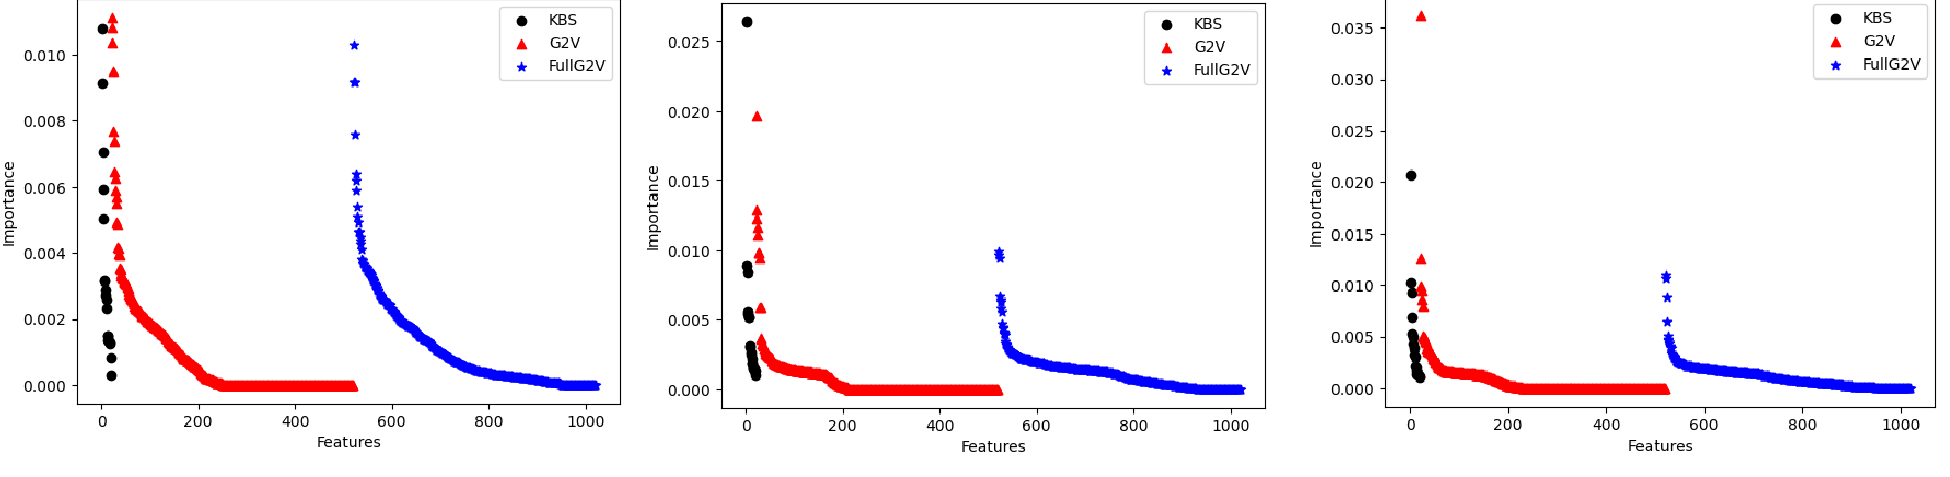
\includegraphics{Images/feature-importance.pdf}
    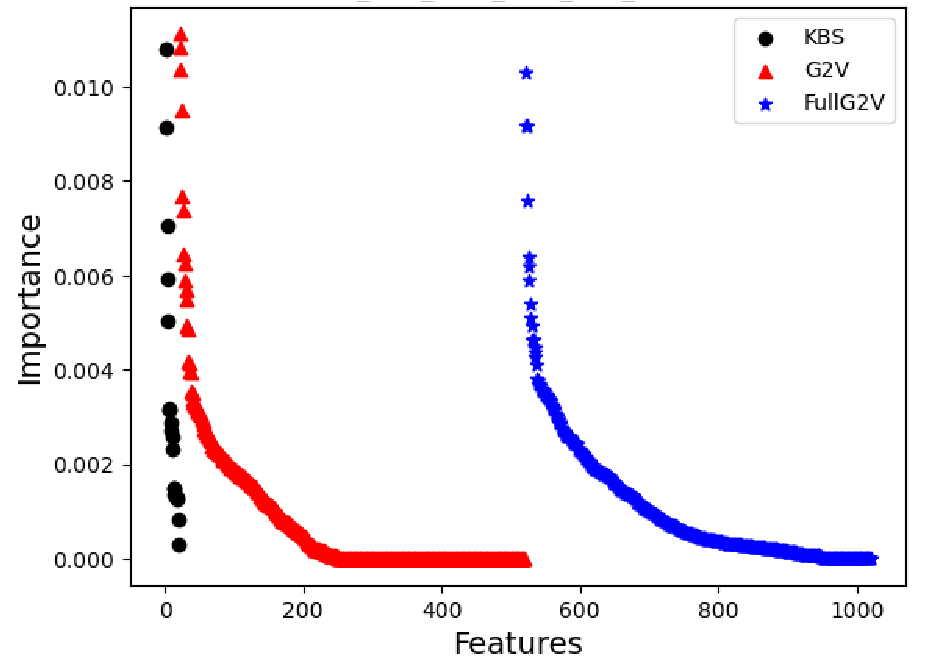
\includegraphics[width=0.6\columnwidth]{Images/in-grid-fi.pdf}
    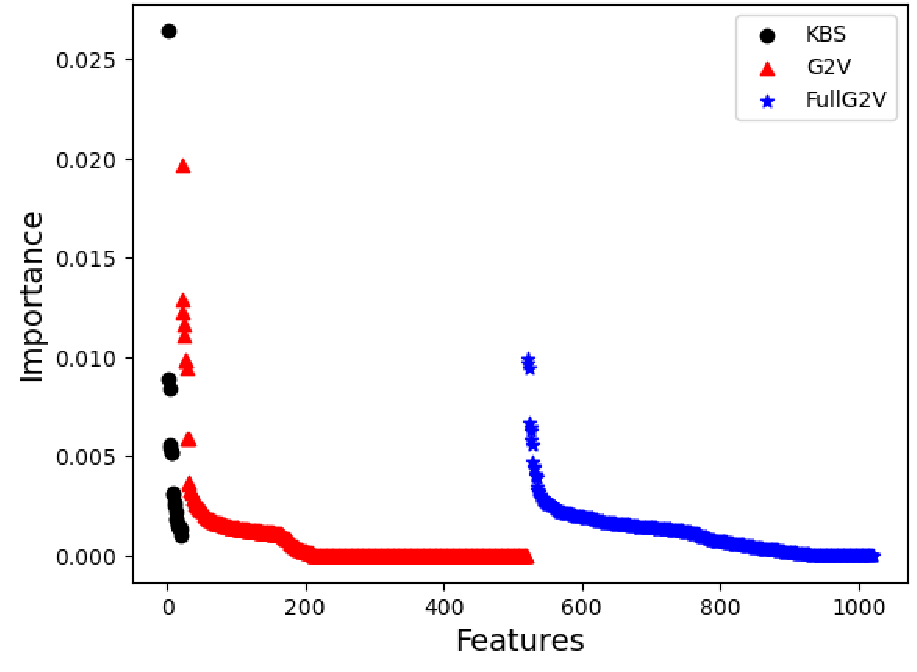
\includegraphics[width=0.6\columnwidth]{Images/in-grid-type-fi.pdf}
    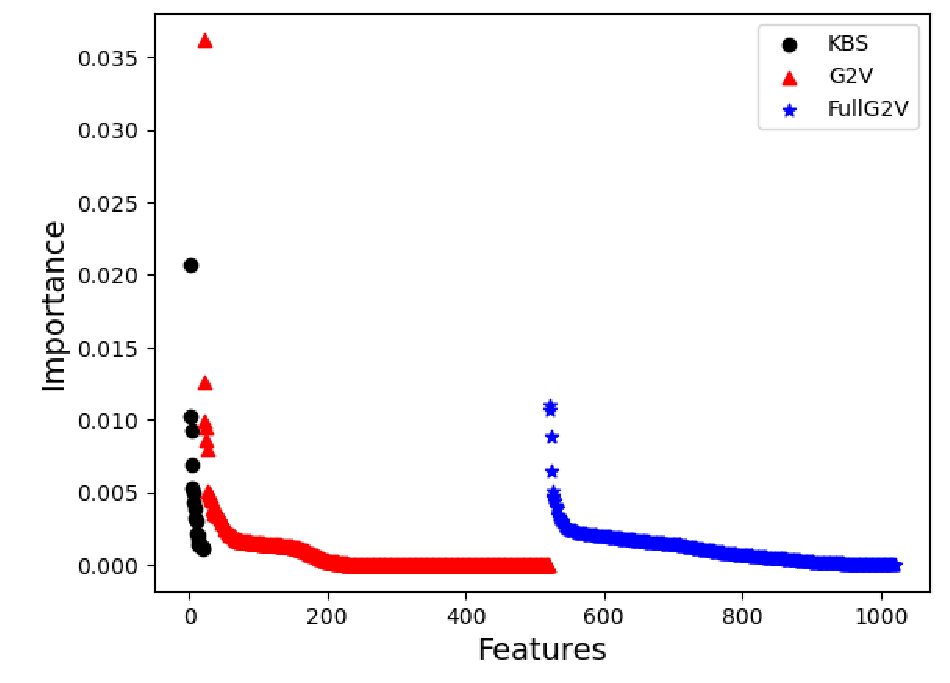
\includegraphics[width=0.6\columnwidth]{Images/between-grid-fi2.pdf}
    \caption{Feature importance for the XGBoost model created for \mapfgas\, in the in-grid (left), in-grid-type (middle), and between-grid (right) setups.}
    \label{fig:model_coefs}
\end{figure*}

Figure \ref{fig:model_coefs} plots a feature importance analysis performed on the prediction models created by \mapfgas\ for each of the AS setups.
The importance of the different features was measured by the coefficient learned for it by the learning algorithm.
The features are listed on the x-axis, where the first 20 features are the \kaduri\ features, the next 500 features are the \gtv\ features, and the last 500 features are the \fgtv\ features. Within each feature family (\kaduri\ ,\gtv\ , and \fgtv\ ), the features are 
% Figure \ref{fig:model_coefs}.
%XGBoost model for the 'in grid split' setup where the scope is "all" maps, is shown in Figure \ref{fig:model_coefs}. \Roni{Can you do the same for all the settings, that is, also for ``in grid-type'' and ``between grid type''?
%~\Roni{Which analysis was done? please explain and add a reference} \Carmel{no real analysis done just plotting the feature's coefs :)} on the best XGBoost model for the 'in grid split' setup where the scope is "all" maps, is shown in Figure \ref{fig:model_coefs}. \Roni{Can you do the same for all the settings, that is, also for ``in grid-type'' and ``between grid type''?
%Also, can you send me these results in a CSV or Excel or something like that?
%I'd like to look at them myself to look for insights} \Carmel{I sent all the 20 csv, once you see all the 20 cases you can choose which ones you want me to plot in same manner}
% The first 500 features are the \fgtv\ features,
% the next 500 features are the \gtv\ features,
% and the remaining 20 are the \kaduri\ features.  %handcrafted features obtained Kaduri's method \cite{kaduri2020algorithm}.


   which corresponds to the successful results of \mapfgas\ .
Another observation is that each feature family includes features  applying feature selection method based on weights may be effective.
When comparing the different AS setups, it    may suggest that additional types of features  may be 

\section{}
We proposed \mapfgas\ , the first practical approach to optiding.
\mapfgas\ uses two encodings of the MAPF problem  diate vicinity.
To work efficiently on new MAPF problems, \mapfgas\ utilizes a modern graph embedding algorithm that does not need a-priori training.
\mapfgas\ also uses hand-crafted MAPF-specific features, as suggested by prior work.
The combination of graph-embedding features and hand-crafted features leads to strong state of the art AS for optimal MAPF.
In an extensive set  that \mapfgas\ significantly outperforms existing baselines almost always.
Our results also highlight that  and can be the focus of future work.
Another impor  MAPFASTER~\cite{alkazzi2022mapfaster}.



\clearpage
\bibliography{ecai}

\end{document}